\documentclass[conference, a4paper, 12pt]{IEEEtran}

\IEEEoverridecommandlockouts

\pdfinterwordspaceon
\input{glyphtounicode}
\pdfgentounicode=1

\usepackage[T2A, T1]{fontenc}
\usepackage[utf8]{inputenc}
\usepackage[final]{microtype}
\usepackage[croatian, french, german, italian, ukrainian, main = british]{babel}

\usepackage[usenames, dvipsnames, svgnames, x11names, table]{xcolor}

\usepackage{amsbsy}
\usepackage{amsmath}
\usepackage{amssymb}
\usepackage{amstext}
\usepackage{amsthm}
\usepackage{listings}
\usepackage{mathtools}
\usepackage[nosepfour]{numprint}
    \npthousandsep{\,}
    \npdecimalsign{\symbol{"002C}}
    \npproductsign{\ensuremath{\cdot}}
    \npunitseparator{\,}
\usepackage{pgfplots}
\usepackage{pgfplotstable}
    \pgfplotsset{%
        compat = newest,
        layers/axis lines on top/.define layer set = {%
            axis background,
            axis grid,
            pre main,
            main,
            axis ticks,
            axis tick labels,
            axis lines,
            axis descriptions,
            axis foreground,
        }{/pgfplots/layers/standard}
    }
    \usepgfplotslibrary{colormaps}
    \pgfkeys{/pgf/number format/.cd, use comma, 1000 sep={\,}}
\usepackage[locale = UK, binary-units = true, group-separator = {\,}, group-four-digits = false, output-decimal-marker = \symbol{"002C}]{siunitx}
\usepackage{stackrel}
\usepackage{thmtools}
\usepackage{tikz}
\usepackage{units}

\usepackage[xindy]{imakeidx}
\usepackage[backend = biber, indexing = true, style = numeric, bibstyle = ieee, citestyle = numeric-comp, sorting = nyvt, sortcites = true, giveninits = true, minnames = 1, maxnames = 6, alldates = short, date = year, isbn = false, doi = false, url = true, eprint = true, arxiv = abs]{biblatex}
    \defbibheading{bibliography}[\bibname]{
        \section*{#1}
        \addcontentsline{toc}{section}{#1}
    }
\usepackage{xpatch}

\usepackage{algorithmic}
\usepackage{array}
\usepackage{booktabs}
\usepackage{caption}
\usepackage{csquotes}
    \MakeOuterQuote{"}
\usepackage[british, calc]{datetime2}
    \DTMusemodule{british}{en-GB}
    \DTMlangsetup[en-GB]{ord = raise, monthyearsep = {,\space}}
\usepackage{graphicx}
\usepackage{longtable}
\usepackage{multicol}
\usepackage{multirow}
%\usepackage{musixtex}
\usepackage{subcaption}
\usepackage{tabularx}
\usepackage{tabu}
\usepackage{textcomp}

\usepackage{varioref}
\usepackage{url}
\usepackage[unicode = true]{hyperref}
    \hypersetup{
        pdfstartview = ,
        pdftitle = {Machine Learning Methods for the Prediction of Scores in the Eurovision Song Contest},
        pdfauthor = {Davor Penzar},
        pdfsubject = {Creation of machine learning models for score prediction in the Eurovision Song Contest},
        pdfkeywords = {music information retrieval, computer audition, deep learning, machine learning, convolutional neural networks, Eurovision Song Contest, score prediction, regression}
    }
\usepackage{bookmark}
\usepackage[noabbrev]{cleveref}

\makeindex
\addbibresource{bibliography.bib}

\newcommand*{\positives}[1]{{#1}_{{+}}}

\newcommand*{\naturals}{\mathbb{N}}
\newcommand*{\reals}{\mathbb{R}}

\newcommand*{\intervalcc}[2]{\left[ {#1} , {#2} \right]}
\newcommand*{\intervalco}[2]{\left[ {#1} , {#2} \right)}

\newcommand*{\bigO}{\mathcal{O}}

\newcommand*{\dotprod}[2]{\left\langle {#1} , {#2} \right\rangle}

\newcommand*{\tran}{\mkern-1.5mu \mathsf{T}}
\DeclareMathOperator{\tr}{\mathrm{tr}}

\DeclareMathOperator{\expect}{\mathbb{E}}
\newcommand*{\mean}[1]{\bar{#1}}
\newcommand*{\Mean}[1]{\overline{#1}}
\DeclareMathOperator{\Var}{\mathit{Var}}
\DeclareMathOperator{\sd}{\mathrm{sd}}
\DeclareMathOperator{\Cov}{\mathit{Cov}}
\DeclareMathOperator{\cov}{\mathit{cov}}

\DeclareMathOperator{\interrel}{\mathit{IR}}

\newcommand*{\myurl}[1]{\href{#1}{\texttt{#1}}}

\lstdefinestyle{myprogram}{
    breaklines = true,
    breakatwhitespace = true,
    numbers = left,
    stepnumber = 1,
    numberstyle = {\footnotesize \ttfamily \bfseries},
    tabsize = 4,
    frame = none,
    basicstyle = {\ttfamily},
    stringstyle = {\color{red}},
    keywordstyle = {\bfseries \color{blue}},
    commentstyle = {\itshape \color{gray}},
    showstringspaces = true
}

\title{
    Machine Learning Methods for the Prediction of Scores in the \href{http://eurovision.tv/}{\emph{Eurovision Song Contest}}
    %\thanks{Personally funded.}
}
\author{
    \IEEEauthorblockN{Davor Penzar}
    \IEEEauthorblockA{
        \textit{freelancing data science and machine learning enthusiast} \\
        Zagreb, Croatia \\
        \href{mailto:davor.penzar@gmail.com}{davor.penzar@gmail.com}
    }
}
\date{May \ensuremath{2022}, Zagreb, Croatia}

\begin{document}
    \maketitle

    \begin{abstract}
        This paper proposes a few machine learning methods and possible models for score prediction in the \href{http://eurovision.tv/}{\emph{Eurovision Song Contest}}. The idea is to train a model for predicting mainstream taste in music, which could be useful in music industry if done successfully. To achieve that, the sound is processed using deep convolutional networks, some of which take in extra non-auditory song features.%
        %After the analysis of the results, the models are employed to predict the score of the Croatian candidates for the \ensuremath{2020} edition of the \href{http://eurovision.tv/}{Contest} had it been held.
    \end{abstract}

    \begin{IEEEkeywords}
       music information retrieval, computer audition, deep learning, machine learning, convolutional neural networks, \href{http://eurovision.tv/}{\emph{Eurovision Song Contest}}, score prediction, regression
    \end{IEEEkeywords}

    \section{Introduction}
    \label{sec:introduction}

    There is no doubt the majority of a \emph{logically} grouped---such as dividing by age, mother tongue, level of education etc.---part of the population share some commonalities in their taste in various forms of art. Naturally, such is the case in music. To illustrate this, in a world where each individual would have their own taste in music completely independent of the others', the popularity of songs would be distributed relatively uniformly. This is obviously not the case: for example, one may observe scores and reviews of songs at~\cite{bib:AM}, \emph{WoC} of top charts at~\cite{bib:UKTop100} or views of trending music videos at~\cite{bib:YTTrend}---simultaneously noticeable, on the other hand, is the great domination of just a few music genres\footnote{Similar statistics could be found for books at~\cite{bib:GR}, for movies and TV shows at~\cite{bib:IMDb,bib:RT}\ldots}. Obviously, the sources mentioned are updated frequently, but it is no surprise that the findings are always the same. In fact, even more stable statistics, such as those at~\cite{bib:Cossar2019}, lead to analogous conclusions. After all, music industry would probably not be as profitable as it is (v.\ \cite{bib:Statista2021}) if the \emph{common taste} did not exist.

    \par

    The phenomenon is not a novelty, either. One could read some interesting facts about the $ 19 $\textsuperscript{th} century pianist virtuoso and composer \foreignlanguage{german}{Franz Liszt}'s popularity at~\cite{bib:Vincent2019} or enjoy the $ 1984 $ M.\ Forman's and P.\ Shaffer's movie \emph{Amadeus} displaying, although dramatically and comically amended, the glorious life and tragic death of the famous $ 18 $\textsuperscript{th} century composer \foreignlanguage{german}{Wolfgang Amadeus Mozart}. Surely we may rely on the idea that the phenomenon will continue on in the future as well.

    \par

    What makes a song (a musically-lyrical piece) a \emph{hit} could be analysed through music theory, literature, linguistics, sociology and other scientific aspects, but that will not be done in this paper. Rather, the idea of the paper is to train an \emph{alien}, completely oblivious of the aforementioned disciplines and their points of interest in songs and pop culture, to predict how the public would respond to a music piece just by hearing it. Of course, such an ignorant is impossible to find (probably a literal intelligent, sound hearing extraterrestrial alien would be the most applicable candidate), therefore compromises had to be made. Due to the area of knowledge and interest of the author, a machine learning model was chosen as a representation of the \emph{alien} mentioned above.

    \par

    If a model proves itself successful, it might be used in music industry to filter out most promising song writers, authors, performers, records and albums, ultimately to boost a record label's business. Not only could this be done faster than by a human, but the process would also be cheaper. Some may argue against this; nevertheless the paper should primarily be viewed as an intellectual exercise in music information retrieval, computer audition and other close fields. However, the author's personal point of view on the possible repercussions of employment of the models in actual music industry is given in the conclusion, section~\ref{subsec:significance_of_computer_aided_art_form}.

    \par

    \subsection{Related Works}
    \label{subsec:related_works}

    As stated in a popular science article at~\cite{bib:Fagella2019}, \href{http://spotify.com/}{\emph{Spotify}} predicts music taste by comparing the user's favourite songs with other users' playlists ($ k $ nearest neighbours or a similar, more complex model). Successful or not, the method does not operate on actual auditory features of songs that the final user enjoys or dislikes but it assumes the same \emph{common taste} on which this paper is based. On the other hand, authors in~\cite{bib:Oord2013} correlated audio features to individuals' preferences in songs, which is very close to the idea of this project. Similar research was conducted at~\cite{bib:McFee2012}. Another popular science article at~\cite{bib:Roza2019} states that not only could a machine learn artistic aesthetics\footnote{In the opinion of this paper's author, art is not solely about aesthetics, and sometimes it is not about aesthetics at all---it all depends on the art form, style and the artist's idea.}, but it could also generate art. The article then references an interesting music analysis and composition model proposed in~\cite{bib:Manaris2007}. On the other hand, visual aesthetics prediction seems to have been developed more thoroughly as seen, for example, at~\cite{bib:Lu2014,bib:Malu2017}.

    \par

    However, machine learning has been extensively employed in audio processing and music information retrieval for classification and tagging purposes: e.~g.\ at~\cite{bib:Hoffman2009,bib:Lee2009,bib:Hamel2010,bib:Dielman2011,bib:Pons2018,bib:Pons2019}. Nonetheless, the author of this paper strongly believes that tags and other objective classes observed are related to listeners' taste and preferences. As a result, the models explained in the aforementioned sources were studied for the purpose of this project.

    \par

    Concerning the \href{http://eurovision.tv/}{\emph{Eurovision Song Contest}}, artificial intelligence and machine learning, the connection has already been made. In $ 2019 $ a song has been created by a machine after learning from a number of \href{http://eurovision.tv/}{\emph{Eurovision}} songs, as described at~\cite{bib:Shapira2019,bib:Drake2019,bib:Ackerman2019}. A year later, in $ 2020 $, an artificial intelligence song contest was held, available at~\cite{bib:VPROAI2020,bib:VPROAIWin2020}. The contest was even announced by \href{http://eurovision.tv/}{\emph{Eurovision}} at~\cite{bib:ESCAI2020}.

    \par

    \subsection{The Choice of the \href{http://eurovision.tv/}{\emph{Eurovision Song Contest}}}
    \label{subsec:the_choice_of_the_eurovision_song_contest}

    The \href{http://eurovision.tv/}{\emph{Eurovision Song Contest} (\emph{ESC})} was chosen as the measurement of the popularity of songs because of its $ 6 $ decades long continuous history (except for the $ 2020 $ edition due to the COVID-$ 19 $ pandemic---v.\ \cite{bib:EVWScores,bib:ESC2020}) and the easily understood scoring system. Unlike measuring popularity of songs by assigning scores to their positions in top charts, numbers of sales and other implicit indicators, the scoring system of the \href{http://eurovision.tv/}{\emph{ESC}} already displays numerically valued popularity of the competing songs expressed through the audience's and the jury's votes. Also, all songs in a single edition of the \href{http://eurovision.tv/}{Contest} had been introduced roughly at the same time and had been available to be listened to approximately the same amount of time, meaning all of them had somewhat equal chance of having their popularity faded out by the time of the \href{http://eurovision.tv/}{Contest}. Finally, local music stars are not necessarily popular abroad, hence songs' scores might be---and, for the purpose of this paper, they hopefully are---independent of artists' popularity.

    \par

    On the other hand, by checking individual scores at~\cite{bib:Okhuijsen2019} (or by watching the \href{http://eurovision.tv/}{\emph{ESC}} over the years) one could notice that some neighbouring or mutually friendly countries usually give each other high points, probably regardless of their actual enjoyment of contestants (songs). Such bias disrupts the idea that the popularity of a song could be predicted merely by analysing how it sounds, indicating that some additional features might have to be introduced. Besides the country of origin of the song, the features may include the language in which the lyrics are, the category of the performer (a solo singer or a band), the performer's sex (or the sex of the lead singer in case of a band) and other easily deducible information. In the end, the author believes that the number of voting countries and the fact that all countries' votes are of equal weights \emph{smooth out} the noise in scores.

    \par

    Of all the songs competing in the \href{http://eurovision.tv/}{\emph{ESC}}, only songs from years $ 1957 $--$ 2019 $ were used because, as mentioned at~\cite{bib:EVWScores}, voting was secret in $ 1956 $ and the scores were not published, plus, in the year $ 2020 $ the \href{http://eurovision.tv/}{Contest} was not held. From the years observed, only the songs and scores from finals (if semifinal round(s) existed) were used because semifinals' and finals' scores are, obviously, not comparable.

    \par

    \section{Dataset}
    \label{sec:dataset}

    Unfortunately, a complete dataset did not exist beforehand and had to be created manually. The main resources were:
    \begin{itemize}
        \item songs from \href{http://youtube.com/}{\emph{YouTube}}, most notably from~\cite{bib:YTESC},
        \item scores by countries from~\cite{bib:Okhuijsen2019,bib:Flecht2020,bib:EVWScores},
        \item extra features from~\cite{bib:Flecht2020,bib:EVWScores} and  \href{http://wikipedia.org/}{\emph{Wikipedia}}.
    \end{itemize}
    It is obvious that the acquired dataset is not verifiable and it may not be completely correct. Also, due to legal reasons---unauthorised distribution of copyrighted music---the author is not able to share their dataset with others. Even the \emph{transformed} dataset (extracted features used as the input of the models, split into \emph{windows} of a consistent format/shape, along with extra features and scores) would be difficult to share because of its size measuring in tens of gibibytes ($ \si{\gibi \byte} $).

    \par

    \subsection{Regional Division of the Contestant Countries}
    \label{subsec:regional_division_of_the_contestant_countries}

    \par

    The country of origin as a non-auditory feature of songs seems to be \emph{too granular} and \emph{too sparse} as a country might have competed in the \href{http://eurovision.tv/}{Contest} only once in a decade. As a result, if the country has never appeared in the training dataset of a model depending on the feature, its score cannot be predicted by the model. To avoid such problems, countries may be grouped into regions according to some geographical, political, linguistic and cultural similarities or differences. While partitioning, regions defined by sources at~\cite{bib:EUEV,bib:CIAFB} were studied, but the final regions are not perfectly aligned with either of the two divisions.

    \par

    European countries appearing in the dataset are divided into $ 6 $ regions which, according to geographical locations, may be named as:
    \begin{itemize}
        \item Central Europe: Austria, Czechia, Germany, Hungary, Poland, Slovakia,
        \item Northern Europe: Denmark, Finland, Iceland, Norway, Sweden,
        \item Western Europe: Belgium, France, Ireland, Luxembourg, Monaco, Netherlands, Switzerland, United Kingdom,
        \item Southern Europe: Cyprus, Greece, Italy, Malta, Portugal, San Marino, Spain,
        \item South-Eastern Europe: Albania, Bosnia and Herzegovina, Bulgaria, Croatia, FYR Macedonia, Montenegro, North Macedonia, Romania, Serbia, Serbia and Montenegro, Slovenia, Yugoslavia,
        \item Eastern Europe: Belarus, Estonia, Latvia, Lithuania, Moldova, Russia, Ukraine.
    \end{itemize}
    Additionally, non-European countries (or those not always considered European) are grouped into their own, seventh group: Armenia, Azerbaijan, Georgia, Israel, Morocco, Turkey. Such division is displayed in figure~\ref{fig:regional_division_of_europe} (some European countries not appearing in the dataset are also assigned to a region and coloured for the completeness of the map).

    \par

    \begin{figure}[tbhp!]
        \centering
        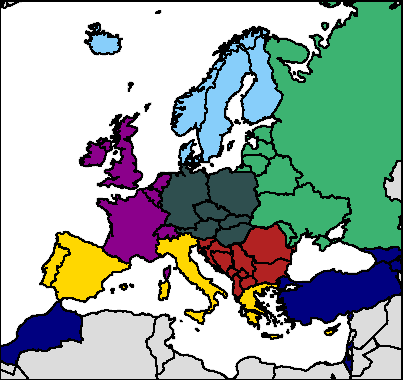
\includegraphics{regions.pdf}
        \captionsetup{singlelinecheck = off}
        \caption[Regional division of Europe]{%
            Regional division of Europe used in the project:
            \begin{itemize}
                \item[\textcolor{DarkSlateGrey}{$ {\blacksquare} $}] Central Europe
                \item[\textcolor{LightSkyBlue}{$ {\blacksquare} $}] Northern Europe
                \item[\textcolor{DarkMagenta}{$ {\blacksquare} $}] Western Europe
                \item[\textcolor{Gold}{$ {\blacksquare} $}] Southern Europe
                \item[\textcolor{FireBrick}{$ {\blacksquare} $}] South-Eastern Europe
                \item[\textcolor{MediumSeaGreen}{$ {\blacksquare} $}] Eastern Europe
                \item[\textcolor{Navy}{$ {\blacksquare} $}] Other
            \end{itemize}
            Countries \colorbox{Gainsboro}{coloured lightly grey} are not assigned to any region/group (they are irrelevant for the dataset).}
        \label{fig:regional_division_of_europe}
    \end{figure}

    \par

    Although Australia is clearly a geographical outsider, it is assigned to Western Europe region because of the economic, political, cultural and linguistic relations to other countries from the region, as opposed to countries from the \emph{non-European} group of countries. Similarly, Slovenia and Croatia were the most questionable countries amongst the European countries. They may be assigned to Central Europe region because of historic and cultural affiliations to rulers from the Central and the Southern Europe\footnote{Of course, in the most recent period both of the countries were parts of Yugoslavia---the kingdom and the socialist federal republic---but for a great part of the second millennium the border of the Ottoman Empire stayed just south of Croatian territories.}, as well as the predominant Roman Catholic religion, while other countries in the South-Eastern region have stronger eastern and south-eastern influences (e.~g.\ Russia, Ottoman Empire). Impacts on culture and religion are certainly present in folklore and ultimately in popular music, but a stronger coherence in terms of the \href{http://eurovision.tv/}{Contest} appears to be between Croatia, Slovenia and other countries from the chosen region when observing voting results at~\cite{bib:Okhuijsen2019,bib:Flecht2020,bib:EVWScores}. After all, the main purpose of the feature is to overcome possible noise in scores caused by biased votes.

    \par

    \subsection{Sound Preprocessing}
    \label{subsec:sound_preprocessing}

    The preprocessing of raw input songs was done simultaneously with the construction of the dataset. Naturally, songs were originally saved as audio files on a computer. A series of \href{http://docs.python.org/3/}{\emph{Python}} programs was then run to extract the dataset from the files.

    \par

    Each song passed a few steps first:
    \begin{enumerate}
        \item it was loaded as a \href{http://numpy.org/doc/stable/reference/generated/numpy.ndarray.html}{\emph{NumPy} \lstinline[style = myprogram, language = Python]{ndarray}} using \href{http://librosa.org/doc/latest/generated/librosa.load.html}{\emph{libROSA} \lstinline[style = myprogram, language = Python]{load} function} as a mono audio signal in a predefined fixed sample rate,
        \item zero-crossing rate (ZCR) was computed from the audio signal using \href{http://librosa.org/doc/latest/generated/librosa.feature.zero_crossing_rate.html}{\emph{libROSA} \lstinline[style = myprogram, language = Python]{feature.zero_crossing_rate} function},
        \item the audio signal (time series) was split into harmonic and percussive components using \href{http://librosa.org/doc/latest/generated/librosa.effects.hpss.html}{\emph{libROSA} \lstinline[style = myprogram, language = Python]{effects.hpss} function},
        \item constant-Q chromagram was computed from the harmonic component using \href{http://librosa.org/doc/latest/generated/librosa.feature.chroma_cqt.html}{\emph{libROSA} \lstinline[style = myprogram, language = Python]{feature.chroma_ctq} function},
        \item tempogram was computed from the percussive component using \href{http://librosa.org/doc/latest/generated/librosa.feature.tempogram.html}{\emph{libROSA} \lstinline[style = myprogram, language = Python]{feature.tempogram} function},
        \item mel-frequency cepstrum (MFC) was computed from the original audio signal using \href{http://librosa.org/doc/latest/generated/librosa.feature.mfcc.html}{\emph{libROSA} \lstinline[style = myprogram, language = Python]{feature.mfcc} function},
        \item the $ 1 $\textsuperscript{st} and the $ 2 $\textsuperscript{nd} derivative $ \Delta $-features were computed from the MFC using \href{http://librosa.org/doc/latest/generated/librosa.feature.delta.html}{\emph{libROSA} \lstinline[style = myprogram, language = Python]{feature.delta}} function.
    \end{enumerate}
    Of all the data mentioned above, only ZCR, chromagram, tempogram, MFC, $ \Delta $-MFC and $ \Delta^{2} $-MFC features were used in the rest of the program. More about the features and their extraction is available at~\cite{bib:McFee2015}.

    \par

    After the features were computed, the first and last $ 10 $ seconds from each song were disregarded (cut out). The reason for this is to avoid using \emph{intros} and \emph{outros} of songs for score prediction since these parts can be very monotone and generic even if middle parts, such as the chorus, are not. Also, a constant signal of magnitude $ 0 $---or even the noise from the live performance (e.~g.\ applause)---might be present at the very beginning or the end of an audio file due to imprecise trimming\footnote{In fact, the author later discovered that some audio files had even longer non-musical beginnings and ends. However, this was taken as an acceptable risk because manual correction of $ 1308 $ audio files was considered too much painstaking work for a single volunteering author, and cutting more than $ \SI{10}{\second} $ seemed as discarding too much valuable information from the properly trimmed samples.}. All possible $ 10 $ second long excerpts (\emph{windows}) of the rest of the song were then extracted\footnote{In reality there are infinitely many $ 10 $ second windows (or, at least, $ 3 \cdot \SI{60}{\second} / t_{\text{P}} \approx \numprint{32.3} \cdot 10^{45} $ windows in a $ 3 $ minute song, where $ t_{\text{P}} $ is the Planck time), but only discrete time points corresponding to the time points of columns of the chromagram, tempogram and MFCC matrices were used.}, and \emph{the most diverse sample} of size $ n $ of them was used. The number $ n \in \naturals $, $ n > 1 $, was fixed and the same for all songs, and \emph{the most diverse sample} was found by conducting the process explained in the appendix, section~\ref{subsec:variance_and_standard_deviation_of_a_multidimensional_sample}, on mel-frequency cepstral coefficient (MFCC) matrices.

    \par

    The choice of the most diverse subsample was made to ensure all different parts of each song were included, and that they were all included in the same extent. Moreover, sampling was done in such a way to maximise diversity (variance) of all observations within a single year of competition. Thus, ideally, each song provided something \emph{new}, something different from other songs to make it easier for the model to distinguish why exactly it should receive the score it received.

    \par

    All hyperparameters (e.~g.\ sample rate, number of MFCCs{\ldots}) were the same for all songs, resulting in a consistent shape of features, regardless of the song from which the windows originated. Furthermore, as the number $ n $ mentioned above was the same for all songs, each song was represented by the same number of observations (windows) no matter what its original duration had been. The final audio dataset was then composed from all the ZCRs, chromagrams, tempograms, MFCs, $ \Delta $-MFCs and $ \Delta^{2} $-MFCs on the chosen windows from all songs. Also, for each window in the final dataset the number $ p \in \intervalcc{0}{1} $, corresponding to the window's middle point's relative position (beginning of the window plus $ 5 $ seconds) in the song, acknowledging the $ 20 $ seconds cut out from the beginning and the end of the song, was saved.

    \par

    \subsection{Splitting the Dataset into Trainig and Validation Datasets}
    \label{subsec:splitting_the_dataset_into_training_and_validation_datasets}

    As the title of the section suggests, no testing dataset was used---at least no explicit one. This shall be explained later, but a model for predicting scores in the year $ y $ is trained and validated on observations from years preceding the year $ y $, i.~e.\ on years $ y - 1 , y - 2 , \dotsc , y - n , \dotsc $, and then, after being fully constructed (trained), it is tested on all observations in the year $ y $. The training and validation datasets, on the other hand, were constructed for each year independently of other years.

    \par

    To split the dataset in a given year into a training and a validation dataset, the observations from the year were split into parts of sizes roughly $ \unit[75]{\%} : \unit[25]{\%} $ of the original (complete) year's dataset; the training set was then chosen as the larger one. However, to avoid the possibility of a classification model \emph{sneaking into} regression models, this was done by splitting observations (windows of songs) in such a manner that each song is completely in either the training or the validation dataset. Otherwise, if a song's windows were simultaneously in the training and the validation datasets, a model could unintentionally be trained to recognise the song from the features and output its score, without modelling a real and useful regression between the features and the score.

    \par

    In order to optimally split observations in each year, the objective was to keep the diversity of observations in the training and validation datasets from the original (complete) year's dataset. Similarly to the generation of windows, the diversity of MFCs was observed; however, this time the diversity (variance) of scores was observed as well. \emph{To keep} the diversity means to minimise the absolute difference between the subsample's diversity and the original sample's diversity; here there were two differences to minimise (the training and the validation datasets'). The process of finding the optimal split is explained in the appendix, section~\ref{subsec:variance_and_standard_deviation_of_a_multidimensional_sample}.

    \par

    \par

    \section{Exploratory Analysis}
    \label{sec:exploratory_analysis}

    The exploratory analysis shall only be focused on scores, quantities and auditory features. Non-auditory features are considered as merely auxiliary information, and not something on which one should focus when studying the problem of the paper. The dataset included information from $ 62 $ (finals) editions of the \href{http://eurovision.tv/}{Contest} (years $ 1957 $--$ 2019 $) with $ 52 $ contestants-countries, by differentiating countries such as Yugoslavia from Serbia and Montenegro or F.~Y.~R.~Macednoina from North Macedonia, resulting in total of $ 1308 $ entries. After extracting multiple windows from each competing song, the number of elements in the dataset multiplied.

    \par

    Note that the exploratory analysis was done on the complete dataset, not only on the training part. Normally this would be considered a bad practice, but the author believes it is not the case here. First of all, normalisation of scores, as shown in figures~\labelcref{fig:distribution_of_normalised_scores_over_years,fig:histogram_of_normalised_scores}, is possible without knowing the actual scores since the average score is calculable just by knowing the rules of voting and the number of voting countries. This is comparable to a situation where data is given in various monetary currencies (v.\ subsection~\ref{subsec:scores} to understand why): in order to make the dataset useful, a set of unifying formulas must be available, either explicitly---as a currency conversion table (average scores per year in our case)---or implicitly---as a set of features on which the conversion factors are dependant or to which they are correlated (voting rules and the number of voting countries in our case). Also, if both the training and the validation datasets were constructed as representative samples consistently over the years, all graphs from sections~\labelcref{subsec:scores,subsec:number_of_contestants} would remain visually similar, albeit with values potentially scaled down (e.~g.\ the number of contestants). Second of all, examples of extracted features are shown in figures~\labelcref{fig:audio_time_series_visualisation,fig:ZCR_visualisation,fig:melspectrogram_visualisation,fig:MFC_visualisation,fig:chromagram_visualisation,fig:cylindrical_chromagram_visualisation,fig:tempogram_visualisation} merely to demonstrate how a raw audio is transformed into features for the models' input. It is actually irrelevant if the example is a part of a training set, a validation set, a testing set or unused by models at all---the transformation is possible on any time series (audio or not) of the correct format.

    \par

    \subsection{Scores}
    \label{subsec:scores}

    Let us observe the distribution of scores over the years. The meaning of line colours in figures~\labelcref{fig:distribution_of_scores_over_years,fig:distribution_of_scores_by_count_over_years,fig:distribution_of_normalised_scores_over_years} (their legend) is the following:
    \begin{itemize}
        \item[\textcolor{RoyalBlue}{$ {\blacksquare} $}] the mean and the surrounding symmetric interval of $ 2 $ standard deviations ($ \text{mean} \pm {\sd} $)\footnote{The interval does not have any significant meaning, such as a confidence interval or anything similar. It only shows the magnitude of the standard deviation, implying dispersion of data (scores)---the wider the area, the more dispersed the data is. Note that the width of the area is observed vertically, in the direction of the $ y $-axis, and not perpendicularly to the mean line.},
        \item[\textcolor{FireBrick}{$ {\blacksquare} $}] the minimum,
        \item[\textcolor{DarkOrange}{$ {\blacksquare} $}] the lower quartile,
        \item[\textcolor{Gold}{$ {\blacksquare} $}] the median,
        \item[\textcolor{YellowGreen}{$ {\blacksquare} $}] the upper quartile,
        \item[\textcolor{SeaGreen}{$ {\blacksquare} $}] the maximum, i.~e.\ the winners' scores.
    \end{itemize}
    All of the figures mentioned above, as well as figure~\ref{fig:number_of_contestants_over_years}, display discrete data (one point per year), but points are connected with straight lines to display progression of values.

    \par

    As one could see in figure~\ref{fig:distribution_of_scores_over_years}, scores were much lower in the beginning of the \href{http://eurovision.tv/}{Contest}. They were even lower in the early $ 2000 $s compared to the scores from the $ 2010 $s.

    \par

    \begin{figure}[tbhp!]
        \centering
        \begin{tikzpicture}

	\begin{axis}[
		/pgf/number format/1000 sep = \empty,
		set layers = axis lines on top,
		xlabel = {Year},
		xmin = 1955,
		xmax = 2021,
		ylabel = {Score},
		ymin = -60,
		ymax = 800
	]

		% mean +/- sd
		\path[draw = none, fill = RoyalBlue, opacity = 0.25]
			(1957, 1.68669072444005)
				-- (1957, 18.31330927556)
				-- (1958, 19.0553851381374)
				-- (1959, 16.180614856145)
				-- (1960, 19.2195444572929)
				-- (1961, 18.2381227635103)
				-- (1962, 12.9474215840603)
				-- (1963, 30.5905954558082)
				-- (1964, 21.3125951772971)
				-- (1965, 18.7256483225602)
				-- (1966, 16.475450015964)
				-- (1967, 21.5108644332213)
				-- (1968, 19.01387818866)
				-- (1969, 15.5737479909543)
				-- (1970, 19.5837935310301)
				-- (1971, 101.749549365854)
				-- (1972, 106.059860456291)
				-- (1973, 108.798126102956)
				-- (1974, 16.0827625302982)
				-- (1975, 102.289451967207)
				-- (1976, 104.186323414927)
				-- (1977, 98.7532026890129)
				-- (1978, 103.977111010177)
				-- (1979, 94.4965751817893)
				-- (1980, 99.9642705167146)
				-- (1981, 100.843657026081)
				-- (1982, 99.6399129795101)
				-- (1983, 102.972506220906)
				-- (1984, 96.7083109077797)
				-- (1985, 94.2889637340182)
				-- (1986, 104.223712301668)
				-- (1987, 102.200840328146)
				-- (1988, 99.2092222688077)
				-- (1989, 97.9130006269589)
				-- (1990, 102.991004391883)
				-- (1991, 108.106553130969)
				-- (1992, 101.693144875265)
				-- (1993, 111.556823405924)
				-- (1994, 113.372977765934)
				-- (1995, 100.073528710839)
				-- (1996, 98.3236903073119)
				-- (1997, 113.253205035244)
				-- (1998, 116.465801970041)
				-- (1999, 106.473985525509)
				-- (2000, 108.996163538566)
				-- (2001, 115.036670819586)
				-- (2002, 104.790931860221)
				-- (2003, 110.893855975907)
				-- (2004, 174.658923998197)
				-- (2005, 156.185625766843)
				-- (2006, 176.617287243137)
				-- (2007, 171.596207178916)
				-- (2008, 173.457738545132)
				-- (2009, 180.937544874086)
				-- (2010, 150.926339839563)
				-- (2011, 148.932553319916)
				-- (2012, 176.144606256153)
				-- (2013, 164.899935815121)
				-- (2014, 155.742412671843)
				-- (2015, 189.549106405795)
				-- (2016, 326.840723726438)
				-- (2017, 371.218252551066)
				-- (2018, 316.603099082142)
				-- (2019, 328.999474216253)
				-- (2019, 36.8466796299007)
				-- (2019, 36.8466796299007)
				-- (2018, 67.0892086101655)
				-- (2017, 3.55097821816494)
				-- (2016, 47.9285070427928)
				-- (2015, -17.6972545539432)
				-- (2014, 9.33451040508034)
				-- (2013, 9.10006418487882)
				-- (2012, 11.2400091284621)
				-- (2011, 50.5874466800838)
				-- (2010, 30.0336601604365)
				-- (2009, 13.942455125914)
				-- (2008, 26.0622614548678)
				-- (2007, 31.4037928210836)
				-- (2006, 7.04937942352967)
				-- (2005, 32.3143742331569)
				-- (2004, -0.658923998197352)
				-- (2003, 5.10614402409293)
				-- (2002, 11.2090681397792)
				-- (2001, 0.963329180413957)
				-- (2000, 7.00383646143394)
				-- (1999, 9.52601447449083)
				-- (1998, -0.465801970040573)
				-- (1997, 2.74679496475642)
				-- (1996, 17.6763096926881)
				-- (1995, 15.9264712891607)
				-- (1994, 2.62702223406559)
				-- (1993, 4.44317659407596)
				-- (1992, 14.3068551247349)
				-- (1991, 7.89344686903053)
				-- (1990, 13.0089956081165)
				-- (1989, 18.0869993730411)
				-- (1988, 16.7907777311923)
				-- (1987, 13.7991596718537)
				-- (1986, 11.7762876983321)
				-- (1985, 21.7110362659818)
				-- (1984, 19.2916890922203)
				-- (1983, 13.0274937790935)
				-- (1982, 16.3600870204899)
				-- (1981, 15.1563429739195)
				-- (1980, 16.0357294832854)
				-- (1979, 21.5034248182107)
				-- (1978, 12.0228889898234)
				-- (1977, 17.2467973109871)
				-- (1976, 11.813676585073)
				-- (1975, 13.7105480327928)
				-- (1974, 3.91723746970178)
				-- (1973, 66.495991544103)
				-- (1972, 65.2734728770422)
				-- (1971, 64.5837839674791)
				-- (1970, 1.74953980230326)
				-- (1969, 4.42625200904574)
				-- (1968, 0.986121811340027)
				-- (1967, -1.51086443322134)
				-- (1966, 1.52454998403598)
				-- (1965, -0.725648322560181)
				-- (1964, -3.31259517729711)
				-- (1963, -0.590595455808179)
				-- (1962, -0.947421584060281)
				-- (1961, 1.7618772364897)
				-- (1960, 0.780455542707113)
				-- (1959, 3.81938514385502)
				-- (1958, 0.944614861862583)
				-- (1957, 1.68669072444005)
				-- cycle;

		% mean
		\addplot[RoyalBlue, thin, dotted]
			table {%
				1957	10
				1958	10
				1959	10
				1960	10
				1961	10
				1962	6
				1963	15
				1964	9
				1965	9
				1966	9
				1967	10
				1968	10
				1969	10
				1970	10.6666666666667
				1971	83.1666666666667
				1972	85.6666666666667
				1973	87.6470588235294
				1974	10
				1975	58
				1976	58
				1977	58
				1978	58
				1979	58
				1980	58
				1981	58
				1982	58
				1983	58
				1984	58
				1985	58
				1986	58
				1987	58
				1988	58
				1989	58
				1990	58
				1991	58
				1992	58
				1993	58
				1994	58
				1995	58
				1996	58
				1997	58
				1998	58
				1999	58
				2000	58
				2001	58
				2002	58
				2003	58
				2004	87
				2005	94.25
				2006	91.8333333333333
				2007	101.5
				2008	99.76
				2009	97.44
				2010	90.48
				2011	99.76
				2012	93.6923076923077
				2013	87
				2014	82.5384615384615
				2015	85.9259259259259
				2016	187.384615384615
				2017	187.384615384615
				2018	191.846153846154
				2019	182.923076923077
			};

		% minimum
		\addplot[FireBrick, dashed]
			table {%
				1957	3
				1958	1
				1959	1
				1960	1
				1961	1
				1962	0
				1963	0
				1964	0
				1965	0
				1966	0
				1967	0
				1968	1
				1969	1
				1970	4
				1971	52
				1972	48
				1973	58
				1974	3
				1975	3
				1976	7
				1977	2
				1978	0
				1979	5
				1980	6
				1981	0
				1982	0
				1983	0
				1984	5
				1985	7
				1986	4
				1987	0
				1988	0
				1989	0
				1990	8
				1991	0
				1992	4
				1993	3
				1994	0
				1995	1
				1996	9
				1997	0
				1998	0
				1999	1
				2000	2
				2001	3
				2002	7
				2003	0
				2004	3
				2005	4
				2006	1
				2007	5
				2008	14
				2009	22
				2010	10
				2011	19
				2012	7
				2013	5
				2014	2
				2015	0
				2016	11
				2017	5
				2018	39
				2019	11
			};

		% lower quartile
		\addplot[DarkOrange, dashed]
			table {%
				1957	5.25
				1958	3.5
				1959	4.5
				1960	4
				1961	5.25
				1962	1.5
				1963	1.5
				1964	0.75
				1965	1
				1966	4.5
				1967	3
				1968	2
				1969	5.75
				1970	5
				1971	68.5
				1972	73.5
				1973	74
				1974	4
				1975	19.5
				1976	17.75
				1977	21.75
				1978	13.75
				1979	32.5
				1980	24
				1981	33
				1982	23.75
				1983	27.5
				1984	32.5
				1985	36
				1986	21.25
				1987	26.5
				1988	20
				1989	32.25
				1990	21.75
				1991	16.25
				1992	24.5
				1993	17
				1994	15
				1995	16
				1996	20.5
				1997	22
				1998	16
				1999	17.5
				2000	18
				2001	17
				2002	25.75
				2003	15.5
				2004	17.5
				2005	42
				2006	25.75
				2007	50.5
				2008	47
				2009	40
				2010	41
				2011	63
				2012	46
				2013	20
				2014	35.5
				2015	17
				2016	105
				2017	77
				2018	102.5
				2019	76.25
			};

		% median
		\addplot[Gold]
			table {%
				1957	7.5
				1958	8
				1959	9
				1960	6
				1961	8.5
				1962	3.5
				1963	9
				1964	5
				1965	6.5
				1966	7.5
				1967	7
				1968	8
				1969	9
				1970	8
				1971	82.5
				1972	85
				1973	85
				1974	10
				1975	53
				1976	55
				1977	51
				1978	63
				1979	60
				1980	47
				1981	45.5
				1982	54.5
				1983	47
				1984	39
				1985	56
				1986	50
				1987	53
				1988	58
				1989	50.5
				1990	48.5
				1991	45.5
				1992	47
				1993	42
				1994	48
				1995	68
				1996	57
				1997	39
				1998	36
				1999	38
				2000	42.5
				2001	37
				2002	35
				2003	37.5
				2004	50
				2005	94.5
				2006	56
				2007	90.5
				2008	69
				2009	74
				2010	72
				2011	96
				2012	70.5
				2013	63.5
				2014	63
				2015	39
				2016	143
				2017	124
				2018	169.5
				2019	108
			};

		% upper quartile
		\addplot[YellowGreen, dashed]
			table {%
				1957	9.5
				1958	12.25
				1959	14.5
				1960	11
				1961	12.25
				1962	10
				1963	25.75
				1964	14
				1965	14
				1966	13.5
				1967	10
				1968	15
				1969	14.25
				1970	9
				1971	89.5
				1972	98
				1973	94
				1974	14
				1975	80.5
				1976	79.25
				1977	86.75
				1978	84.5
				1979	78
				1980	90
				1981	78
				1982	83.25
				1983	82.75
				1984	70
				1985	92
				1986	77.25
				1987	82.25
				1988	87
				1989	85
				1990	85.5
				1991	101.75
				1992	82.5
				1993	89
				1994	74
				1995	87.5
				1996	85
				1997	95
				1998	86
				1999	88
				2000	89
				2001	73
				2002	82
				2003	87.75
				2004	122
				2005	139.75
				2006	149.25
				2007	140.5
				2008	138
				2009	120
				2010	141
				2011	120
				2012	111.5
				2013	124.5
				2014	88.75
				2015	104
				2016	244
				2017	261.5
				2018	266.75
				2019	304.25
			};

		% maximum (winners)
		\addplot[SeaGreen, dashed]
			table {%
				1957	31
				1958	27
				1959	21
				1960	32
				1961	31
				1962	26
				1963	42
				1964	49
				1965	32
				1966	31
				1967	47
				1968	29
				1969	18
				1970	32
				1971	128
				1972	128
				1973	129
				1974	24
				1975	152
				1976	164
				1977	136
				1978	157
				1979	125
				1980	143
				1981	136
				1982	161
				1983	142
				1984	145
				1985	123
				1986	176
				1987	172
				1988	137
				1989	137
				1990	149
				1991	146
				1992	155
				1993	187
				1994	226
				1995	148
				1996	162
				1997	227
				1998	172
				1999	163
				2000	195
				2001	198
				2002	176
				2003	167
				2004	280
				2005	230
				2006	292
				2007	268
				2008	272
				2009	387
				2010	246
				2011	221
				2012	372
				2013	281
				2014	290
				2015	365
				2016	534
				2017	758
				2018	529
				2019	498
			};

	\end{axis}

\end{tikzpicture}

        \caption{Distribution of scores over years}
        \label{fig:distribution_of_scores_over_years}
    \end{figure}

    \par

    Of course, one of the reasons why the scores increased over the years may be the increase in the number of contestants, as seen in figure~\ref{fig:number_of_contestants_over_years}. Given a fixed set of rules regarding voting and scoring (independent of the number of contestants), one could expect the scores to be proportional to the number of contestants---after all, by accepting the original idea that the preferability of a song may be predicted, this comes as a natural conclusion (a common taste should exist amongst voters). However, as seen in figure~\ref{fig:distribution_of_scores_by_count_over_years}, which displays the progression of ratios of the score and the number of contestants over the years, the shape of curves is very similar to those in figure~\ref{fig:distribution_of_scores_over_years}---even the measures of central tendency (the mean and the median) are inconsistent. In other words, irregularity of scores' meanings is still present.

    \par

    \begin{figure}[tbhp!]
        \centering
        \begin{tikzpicture}

	\begin{axis}[
		/pgf/number format/1000 sep = \empty,
		set layers = axis lines on top,
		xlabel = {Year},
		xmin = 1955,
		xmax = 2021,
		ylabel = {$ \text{Score} / \text{count} $},
		ymin = -2,
		ymax = 30
	]

		% mean +/- sd
		\path[draw = none, fill = RoyalBlue, opacity = 0.25]
			(1957, 0.168669072444005)
				-- (1957, 1.831330927556)
				-- (1958, 1.90553851381374)
				-- (1959, 1.47096498692227)
				-- (1960, 1.47842649671484)
				-- (1961, 1.13988267271939)
				-- (1962, 0.809213849003768)
				-- (1963, 1.91191221598801)
				-- (1964, 1.33203719858107)
				-- (1965, 1.04031379569779)
				-- (1966, 0.915302778664668)
				-- (1967, 1.26534496666008)
				-- (1968, 1.11846342286235)
				-- (1969, 0.973359249434641)
				-- (1970, 1.63198279425251)
				-- (1971, 5.65275274254746)
				-- (1972, 5.89221446979395)
				-- (1973, 6.39988977076211)
				-- (1974, 0.946044854723425)
				-- (1975, 5.38365536669512)
				-- (1976, 5.78812907860706)
				-- (1977, 5.48628903827849)
				-- (1978, 5.19885555050883)
				-- (1979, 4.97350395693628)
				-- (1980, 5.26127739561656)
				-- (1981, 5.04218285130403)
				-- (1982, 5.5355507210839)
				-- (1983, 5.14862531104532)
				-- (1984, 5.08991110040946)
				-- (1985, 4.96257703863254)
				-- (1986, 5.2111856150834)
				-- (1987, 4.64549274218847)
				-- (1988, 4.72424867946704)
				-- (1989, 4.45059093758904)
				-- (1990, 4.68140929054016)
				-- (1991, 4.91393423322589)
				-- (1992, 4.42144108153327)
				-- (1993, 4.46227293623696)
				-- (1994, 4.53491911063738)
				-- (1995, 4.3510229874278)
				-- (1996, 4.27494305683965)
				-- (1997, 4.53012820140974)
				-- (1998, 4.65863207880162)
				-- (1999, 4.6293037185004)
				-- (2000, 4.54150681410692)
				-- (2001, 5.00159438346026)
				-- (2002, 4.3662888275092)
				-- (2003, 4.26514830676566)
				-- (2004, 7.27745516659156)
				-- (2005, 6.50773440695179)
				-- (2006, 7.35905363513071)
				-- (2007, 7.14984196578818)
				-- (2008, 6.93830954180529)
				-- (2009, 7.23750179496344)
				-- (2010, 6.03705359358254)
				-- (2011, 5.95730213279665)
				-- (2012, 6.77479254831359)
				-- (2013, 6.34230522365851)
				-- (2014, 5.99009279507087)
				-- (2015, 7.02033727428871)
				-- (2016, 12.5707970664015)
				-- (2017, 14.2776250981179)
				-- (2018, 12.1770422723901)
				-- (2019, 12.6538259313943)
				-- (2019, 1.41717998576542)
				-- (2019, 1.41717998576542)
				-- (2018, 2.58035417731406)
				-- (2017, 0.136576085314037)
				-- (2016, 1.84340411703049)
				-- (2015, -0.655453872368267)
				-- (2014, 0.359019630964629)
				-- (2013, 0.350002468649186)
				-- (2012, 0.432308043402387)
				-- (2011, 2.02349786720335)
				-- (2010, 1.20134640641746)
				-- (2009, 0.55769820503656)
				-- (2008, 1.04249045819471)
				-- (2007, 1.30849136754515)
				-- (2006, 0.29372414264707)
				-- (2005, 1.34643225971487)
				-- (2004, -0.0274551665915563)
				-- (2003, 0.196390154772805)
				-- (2002, 0.467044505824133)
				-- (2001, 0.0418838774093024)
				-- (2000, 0.291826519226414)
				-- (1999, 0.414174542369166)
				-- (1998, -0.0186320788016232)
				-- (1997, 0.109871798590257)
				-- (1996, 0.768535204029918)
				-- (1995, 0.69245527344177)
				-- (1994, 0.105080889362624)
				-- (1993, 0.177727063763038)
				-- (1992, 0.622037179336298)
				-- (1991, 0.358793039501387)
				-- (1990, 0.591317982187116)
				-- (1989, 0.822136335138233)
				-- (1988, 0.799560844342488)
				-- (1987, 0.627234530538804)
				-- (1986, 0.588814384916603)
				-- (1985, 1.1426861192622)
				-- (1984, 1.01535205748528)
				-- (1983, 0.651374688954675)
				-- (1982, 0.908893723360548)
				-- (1981, 0.757817148695972)
				-- (1980, 0.84398576227818)
				-- (1979, 1.13175920095846)
				-- (1978, 0.601144449491168)
				-- (1977, 0.958155406165953)
				-- (1976, 0.656315365837388)
				-- (1975, 0.72160779119962)
				-- (1974, 0.23042573351187)
				-- (1973, 3.911528914359)
				-- (1972, 3.62630404872457)
				-- (1971, 3.58798799819328)
				-- (1970, 0.145794983525272)
				-- (1969, 0.276640750565359)
				-- (1968, 0.0580071653729426)
				-- (1967, -0.0888743784247845)
				-- (1966, 0.0846972213353322)
				-- (1965, -0.0403137956977878)
				-- (1964, -0.207037198581069)
				-- (1963, -0.0369122159880112)
				-- (1962, -0.0592138490037676)
				-- (1961, 0.110117327280606)
				-- (1960, 0.060035041746701)
				-- (1959, 0.347216831259547)
				-- (1958, 0.0944614861862583)
				-- (1957, 0.168669072444005)
				-- cycle;

		% mean
		\addplot[RoyalBlue, thin, dotted]
			table {%
				1957	1
				1958	1
				1959	0.909090909090909
				1960	0.769230769230769
				1961	0.625
				1962	0.375
				1963	0.9375
				1964	0.5625
				1965	0.5
				1966	0.5
				1967	0.588235294117647
				1968	0.588235294117647
				1969	0.625
				1970	0.888888888888889
				1971	4.62037037037037
				1972	4.75925925925926
				1973	5.15570934256055
				1974	0.588235294117647
				1975	3.05263157894737
				1976	3.22222222222222
				1977	3.22222222222222
				1978	2.9
				1979	3.05263157894737
				1980	3.05263157894737
				1981	2.9
				1982	3.22222222222222
				1983	2.9
				1984	3.05263157894737
				1985	3.05263157894737
				1986	2.9
				1987	2.63636363636364
				1988	2.76190476190476
				1989	2.63636363636364
				1990	2.63636363636364
				1991	2.63636363636364
				1992	2.52173913043478
				1993	2.32
				1994	2.32
				1995	2.52173913043478
				1996	2.52173913043478
				1997	2.32
				1998	2.32
				1999	2.52173913043478
				2000	2.41666666666667
				2001	2.52173913043478
				2002	2.41666666666667
				2003	2.23076923076923
				2004	3.625
				2005	3.92708333333333
				2006	3.82638888888889
				2007	4.22916666666667
				2008	3.9904
				2009	3.8976
				2010	3.6192
				2011	3.9904
				2012	3.60355029585799
				2013	3.34615384615385
				2014	3.17455621301775
				2015	3.18244170096022
				2016	7.20710059171598
				2017	7.20710059171598
				2018	7.37869822485207
				2019	7.03550295857988
			};

		% minimum
		\addplot[FireBrick, dashed]
			table {%
				1957	0.3
				1958	0.1
				1959	0.0909090909090909
				1960	0.0769230769230769
				1961	0.0625
				1962	0
				1963	0
				1964	0
				1965	0
				1966	0
				1967	0
				1968	0.0588235294117647
				1969	0.0625
				1970	0.333333333333333
				1971	2.88888888888889
				1972	2.66666666666667
				1973	3.41176470588235
				1974	0.176470588235294
				1975	0.157894736842105
				1976	0.388888888888889
				1977	0.111111111111111
				1978	0
				1979	0.263157894736842
				1980	0.315789473684211
				1981	0
				1982	0
				1983	0
				1984	0.263157894736842
				1985	0.368421052631579
				1986	0.2
				1987	0
				1988	0
				1989	0
				1990	0.363636363636364
				1991	0
				1992	0.173913043478261
				1993	0.12
				1994	0
				1995	0.0434782608695652
				1996	0.391304347826087
				1997	0
				1998	0
				1999	0.0434782608695652
				2000	0.0833333333333333
				2001	0.130434782608696
				2002	0.291666666666667
				2003	0
				2004	0.125
				2005	0.166666666666667
				2006	0.0416666666666667
				2007	0.208333333333333
				2008	0.56
				2009	0.88
				2010	0.4
				2011	0.76
				2012	0.269230769230769
				2013	0.192307692307692
				2014	0.0769230769230769
				2015	0
				2016	0.423076923076923
				2017	0.192307692307692
				2018	1.5
				2019	0.423076923076923
			};

		% lower quartile
		\addplot[DarkOrange, dashed]
			table {%
				1957	0.525
				1958	0.35
				1959	0.409090909090909
				1960	0.307692307692308
				1961	0.328125
				1962	0.09375
				1963	0.09375
				1964	0.046875
				1965	0.0555555555555556
				1966	0.25
				1967	0.176470588235294
				1968	0.117647058823529
				1969	0.359375
				1970	0.416666666666667
				1971	3.80555555555556
				1972	4.08333333333333
				1973	4.35294117647059
				1974	0.235294117647059
				1975	1.02631578947368
				1976	0.986111111111111
				1977	1.20833333333333
				1978	0.6875
				1979	1.71052631578947
				1980	1.26315789473684
				1981	1.65
				1982	1.31944444444444
				1983	1.375
				1984	1.71052631578947
				1985	1.89473684210526
				1986	1.0625
				1987	1.20454545454545
				1988	0.952380952380952
				1989	1.46590909090909
				1990	0.988636363636364
				1991	0.738636363636364
				1992	1.06521739130435
				1993	0.68
				1994	0.6
				1995	0.695652173913043
				1996	0.891304347826087
				1997	0.88
				1998	0.64
				1999	0.760869565217391
				2000	0.75
				2001	0.739130434782609
				2002	1.07291666666667
				2003	0.596153846153846
				2004	0.729166666666667
				2005	1.75
				2006	1.07291666666667
				2007	2.10416666666667
				2008	1.88
				2009	1.6
				2010	1.64
				2011	2.52
				2012	1.76923076923077
				2013	0.769230769230769
				2014	1.36538461538462
				2015	0.62962962962963
				2016	4.03846153846154
				2017	2.96153846153846
				2018	3.94230769230769
				2019	2.93269230769231
			};

		% median
		\addplot[Gold]
			table {%
				1957	0.75
				1958	0.8
				1959	0.818181818181818
				1960	0.461538461538462
				1961	0.53125
				1962	0.21875
				1963	0.5625
				1964	0.3125
				1965	0.361111111111111
				1966	0.416666666666667
				1967	0.411764705882353
				1968	0.470588235294118
				1969	0.5625
				1970	0.666666666666667
				1971	4.58333333333333
				1972	4.72222222222222
				1973	5
				1974	0.588235294117647
				1975	2.78947368421053
				1976	3.05555555555556
				1977	2.83333333333333
				1978	3.15
				1979	3.15789473684211
				1980	2.47368421052632
				1981	2.275
				1982	3.02777777777778
				1983	2.35
				1984	2.05263157894737
				1985	2.94736842105263
				1986	2.5
				1987	2.40909090909091
				1988	2.76190476190476
				1989	2.29545454545455
				1990	2.20454545454545
				1991	2.06818181818182
				1992	2.04347826086957
				1993	1.68
				1994	1.92
				1995	2.95652173913043
				1996	2.47826086956522
				1997	1.56
				1998	1.44
				1999	1.65217391304348
				2000	1.77083333333333
				2001	1.60869565217391
				2002	1.45833333333333
				2003	1.44230769230769
				2004	2.08333333333333
				2005	3.9375
				2006	2.33333333333333
				2007	3.77083333333333
				2008	2.76
				2009	2.96
				2010	2.88
				2011	3.84
				2012	2.71153846153846
				2013	2.44230769230769
				2014	2.42307692307692
				2015	1.44444444444444
				2016	5.5
				2017	4.76923076923077
				2018	6.51923076923077
				2019	4.15384615384615
			};

		% upper quartile
		\addplot[YellowGreen, dashed]
			table {%
				1957	0.95
				1958	1.225
				1959	1.31818181818182
				1960	0.846153846153846
				1961	0.765625
				1962	0.625
				1963	1.609375
				1964	0.875
				1965	0.777777777777778
				1966	0.75
				1967	0.588235294117647
				1968	0.882352941176471
				1969	0.890625
				1970	0.75
				1971	4.97222222222222
				1972	5.44444444444444
				1973	5.52941176470588
				1974	0.823529411764706
				1975	4.23684210526316
				1976	4.40277777777778
				1977	4.81944444444444
				1978	4.225
				1979	4.10526315789474
				1980	4.73684210526316
				1981	3.9
				1982	4.625
				1983	4.1375
				1984	3.68421052631579
				1985	4.84210526315789
				1986	3.8625
				1987	3.73863636363636
				1988	4.14285714285714
				1989	3.86363636363636
				1990	3.88636363636364
				1991	4.625
				1992	3.58695652173913
				1993	3.56
				1994	2.96
				1995	3.80434782608696
				1996	3.69565217391304
				1997	3.8
				1998	3.44
				1999	3.82608695652174
				2000	3.70833333333333
				2001	3.17391304347826
				2002	3.41666666666667
				2003	3.375
				2004	5.08333333333333
				2005	5.82291666666667
				2006	6.21875
				2007	5.85416666666667
				2008	5.52
				2009	4.8
				2010	5.64
				2011	4.8
				2012	4.28846153846154
				2013	4.78846153846154
				2014	3.41346153846154
				2015	3.85185185185185
				2016	9.38461538461539
				2017	10.0576923076923
				2018	10.2596153846154
				2019	11.7019230769231
			};

		% maximum (winners)
		\addplot[SeaGreen, dashed]
			table {%
				1957	3.1
				1958	2.7
				1959	1.90909090909091
				1960	2.46153846153846
				1961	1.9375
				1962	1.625
				1963	2.625
				1964	3.0625
				1965	1.77777777777778
				1966	1.72222222222222
				1967	2.76470588235294
				1968	1.70588235294118
				1969	1.125
				1970	2.66666666666667
				1971	7.11111111111111
				1972	7.11111111111111
				1973	7.58823529411765
				1974	1.41176470588235
				1975	8
				1976	9.11111111111111
				1977	7.55555555555556
				1978	7.85
				1979	6.57894736842105
				1980	7.52631578947368
				1981	6.8
				1982	8.94444444444444
				1983	7.1
				1984	7.63157894736842
				1985	6.47368421052632
				1986	8.8
				1987	7.81818181818182
				1988	6.52380952380952
				1989	6.22727272727273
				1990	6.77272727272727
				1991	6.63636363636364
				1992	6.73913043478261
				1993	7.48
				1994	9.04
				1995	6.43478260869565
				1996	7.04347826086957
				1997	9.08
				1998	6.88
				1999	7.08695652173913
				2000	8.125
				2001	8.60869565217391
				2002	7.33333333333333
				2003	6.42307692307692
				2004	11.6666666666667
				2005	9.58333333333333
				2006	12.1666666666667
				2007	11.1666666666667
				2008	10.88
				2009	15.48
				2010	9.84
				2011	8.84
				2012	14.3076923076923
				2013	10.8076923076923
				2014	11.1538461538462
				2015	13.5185185185185
				2016	20.5384615384615
				2017	29.1538461538462
				2018	20.3461538461538
				2019	19.1538461538462
			};

	\end{axis}

\end{tikzpicture}

        \caption{Distribution of scores by count over years}
        \label{fig:distribution_of_scores_by_count_over_years}
    \end{figure}

    \par

    One could standardise scores by subtracting the mean and dividing by the standard deviation ($ X \mapsto \left( X - \expect \left[ X \right] \right) / \sqrt{\Var \left( X \right)} $), but such values would be \emph{even more meaningless} than the original scores: for instance, ratios amongst scores of contestants in the same year would be lost. Also, by predicting such values one could only determine the final ranking list, but not the actual scores. Alternatively, the normalisation of scores could be done by dividing scores by the mean in their respective years (divide scores in the year $ y $ by the mean of all scores in the year $ y $)\footnote{Since the resulting values are not necessarily limited to the interval $ \intervalcc{0}{1} $, the term \emph{normalisation} may not be entirely correct. However, as the mean is set to a constant value of $ 1 $ by scaling, this term was chosen to describe the transformation at hand.}. As seen in figure~\ref{fig:distribution_of_normalised_scores_over_years}, this produces much more consistent scoring over the years compared to the previous two graphs, by simultaneously keeping ratios amongst scores in the same year. The meaning of normalised scores may also be considered consistent: scoring $ 2 $ normalised points means the same regardless of the year---except in the early $ 1970 $s when scores were much more densely distributed, probably because of rules explained at~\cite{bib:EVWScores}. Also, predicting such values is interpretable: by knowing the rules regarding voting and scoring, as well as the number of voting countries in a given year, one could easily calculate the actual predicted score of a song from the predicted normalised score.

    \par

    \begin{figure}[tbhp!]
        \centering
        \begin{tikzpicture}

	\begin{axis}[
		/pgf/number format/1000 sep = \empty,
		set layers = axis lines on top,
		xlabel = {Year},
		xmin = 1955,
		xmax = 2021,
		ylabel = {Normalised score},
		ymin = -0.75,
		ymax = 6
	]

		% mean +/- sd
		\path[draw = none, fill = RoyalBlue, opacity = 0.25]
			(1957, 0.168669072444005)
				-- (1957, 1.831330927556)
				-- (1958, 1.90553851381374)
				-- (1959, 1.6180614856145)
				-- (1960, 1.92195444572929)
				-- (1961, 1.82381227635103)
				-- (1962, 2.15790359734338)
				-- (1963, 2.03937303038721)
				-- (1964, 2.36806613081079)
				-- (1965, 2.08062759139558)
				-- (1966, 1.83060555732934)
				-- (1967, 2.15108644332213)
				-- (1968, 1.901387818866)
				-- (1969, 1.55737479909543)
				-- (1970, 1.83598064353407)
				-- (1971, 1.22344147534093)
				-- (1972, 1.23805284579328)
				-- (1973, 1.2413209018458)
				-- (1974, 1.60827625302982)
				-- (1975, 1.76361124081392)
				-- (1976, 1.79631592094702)
				-- (1977, 1.70264142567264)
				-- (1978, 1.79270881052029)
				-- (1979, 1.62925129623775)
				-- (1980, 1.7235219054606)
				-- (1981, 1.73868374182898)
				-- (1982, 1.71792953412948)
				-- (1983, 1.77538803829149)
				-- (1984, 1.66738467082379)
				-- (1985, 1.62567178851756)
				-- (1986, 1.79696055692531)
				-- (1987, 1.76208345393356)
				-- (1988, 1.71050383222082)
				-- (1989, 1.68815518322343)
				-- (1990, 1.77570697227385)
				-- (1991, 1.86390608846499)
				-- (1992, 1.7533300840563)
				-- (1993, 1.92339350699869)
				-- (1994, 1.95470651320577)
				-- (1995, 1.72540566742826)
				-- (1996, 1.69523603978124)
				-- (1997, 1.95264146612489)
				-- (1998, 2.00803106844898)
				-- (1999, 1.83575837112947)
				-- (2000, 1.87924419894079)
				-- (2001, 1.98339087619976)
				-- (2002, 1.80674020448657)
				-- (2003, 1.91196303406736)
				-- (2004, 2.00757383905974)
				-- (2005, 1.65714191795059)
				-- (2006, 1.92323724765666)
				-- (2007, 1.69060302639326)
				-- (2008, 1.73875038637863)
				-- (2009, 1.85691240634325)
				-- (2010, 1.66806299557431)
				-- (2011, 1.49290851363188)
				-- (2012, 1.88003274329228)
				-- (2013, 1.89540156109335)
				-- (2014, 1.88690714327489)
				-- (2015, 2.20595942799848)
				-- (2016, 1.74422389509183)
				-- (2017, 1.9810497878341)
				-- (2018, 1.65029682761341)
				-- (2019, 1.79856735273814)
				-- (2019, 0.201432647261863)
				-- (2019, 0.201432647261863)
				-- (2018, 0.349703172386589)
				-- (2017, 0.0189502121659048)
				-- (2016, 0.255776104908172)
				-- (2015, -0.205959427998477)
				-- (2014, 0.113092856725111)
				-- (2013, 0.104598438906653)
				-- (2012, 0.119967256707723)
				-- (2011, 0.507091486368122)
				-- (2010, 0.331937004425691)
				-- (2009, 0.143087593656753)
				-- (2008, 0.261249613621369)
				-- (2007, 0.309396973606735)
				-- (2006, 0.0767627523433358)
				-- (2005, 0.342858082049411)
				-- (2004, -0.00757383905973952)
				-- (2003, 0.0880369659326368)
				-- (2002, 0.193259795513434)
				-- (2001, 0.0166091238002408)
				-- (2000, 0.120755801059206)
				-- (1999, 0.164241628870532)
				-- (1998, -0.00803106844897505)
				-- (1997, 0.0473585338751106)
				-- (1996, 0.30476396021876)
				-- (1995, 0.274594332571736)
				-- (1994, 0.0452934867942342)
				-- (1993, 0.0766064930013098)
				-- (1992, 0.246669915943704)
				-- (1991, 0.136093911535009)
				-- (1990, 0.224293027726148)
				-- (1989, 0.311844816776571)
				-- (1988, 0.289496167779177)
				-- (1987, 0.237916546066443)
				-- (1986, 0.203039443074691)
				-- (1985, 0.374328211482445)
				-- (1984, 0.332615329176213)
				-- (1983, 0.224611961708508)
				-- (1982, 0.282070465870515)
				-- (1981, 0.261316258171025)
				-- (1980, 0.276478094539404)
				-- (1979, 0.370748703762253)
				-- (1978, 0.207291189479713)
				-- (1977, 0.297358574327364)
				-- (1976, 0.203684079052983)
				-- (1975, 0.236388759186083)
				-- (1974, 0.391723746970178)
				-- (1973, 0.758679098154195)
				-- (1972, 0.761947154206719)
				-- (1971, 0.776558524659067)
				-- (1970, 0.164019356465931)
				-- (1969, 0.442625200904574)
				-- (1968, 0.0986121811340027)
				-- (1967, -0.151086443322134)
				-- (1966, 0.169394442670664)
				-- (1965, -0.0806275913955756)
				-- (1964, -0.36806613081079)
				-- (1963, -0.0393730303872121)
				-- (1962, -0.15790359734338)
				-- (1961, 0.17618772364897)
				-- (1960, 0.0780455542707111)
				-- (1959, 0.381938514385502)
				-- (1958, 0.0944614861862583)
				-- (1957, 0.168669072444005)
				-- cycle;

		% mean
		\addplot[RoyalBlue, thin, dotted]
			table {%
				1957	1
				1958	1
				1959	1
				1960	1
				1961	1
				1962	1
				1963	1
				1964	1
				1965	1
				1966	1
				1967	1
				1968	1
				1969	1
				1970	1
				1971	1
				1972	1
				1973	1
				1974	1
				1975	1
				1976	1
				1977	1
				1978	1
				1979	1
				1980	1
				1981	1
				1982	1
				1983	1
				1984	1
				1985	1
				1986	1
				1987	1
				1988	1
				1989	1
				1990	1
				1991	1
				1992	1
				1993	1
				1994	1
				1995	1
				1996	1
				1997	1
				1998	1
				1999	1
				2000	1
				2001	1
				2002	1
				2003	1
				2004	1
				2005	1
				2006	1
				2007	1
				2008	1
				2009	1
				2010	1
				2011	1
				2012	1
				2013	1
				2014	1
				2015	1
				2016	1
				2017	1
				2018	1
				2019	1
			};

		% minimum
		\addplot[FireBrick, dashed]
			table {%
				1957	0.3
				1958	0.1
				1959	0.1
				1960	0.1
				1961	0.1
				1962	0
				1963	0
				1964	0
				1965	0
				1966	0
				1967	0
				1968	0.1
				1969	0.1
				1970	0.375
				1971	0.625250501002004
				1972	0.560311284046693
				1973	0.661744966442953
				1974	0.3
				1975	0.0517241379310345
				1976	0.120689655172414
				1977	0.0344827586206897
				1978	0
				1979	0.0862068965517241
				1980	0.103448275862069
				1981	0
				1982	0
				1983	0
				1984	0.0862068965517241
				1985	0.120689655172414
				1986	0.0689655172413793
				1987	0
				1988	0
				1989	0
				1990	0.137931034482759
				1991	0
				1992	0.0689655172413793
				1993	0.0517241379310345
				1994	0
				1995	0.0172413793103448
				1996	0.155172413793103
				1997	0
				1998	0
				1999	0.0172413793103448
				2000	0.0344827586206897
				2001	0.0517241379310345
				2002	0.120689655172414
				2003	0
				2004	0.0344827586206897
				2005	0.0424403183023873
				2006	0.0108892921960073
				2007	0.0492610837438424
				2008	0.140336808340016
				2009	0.225779967159278
				2010	0.1105216622458
				2011	0.190457097032879
				2012	0.0747126436781609
				2013	0.0574712643678161
				2014	0.0242311276794035
				2015	0
				2016	0.0587027914614121
				2017	0.0266830870279146
				2018	0.203287890938252
				2019	0.06013456686291
			};

		% lower quartile
		\addplot[DarkOrange, dashed]
			table {%
				1957	0.525
				1958	0.35
				1959	0.45
				1960	0.4
				1961	0.525
				1962	0.25
				1963	0.1
				1964	0.0833333333333333
				1965	0.111111111111111
				1966	0.5
				1967	0.3
				1968	0.2
				1969	0.575
				1970	0.46875
				1971	0.823647294589178
				1972	0.857976653696498
				1973	0.844295302013423
				1974	0.4
				1975	0.336206896551724
				1976	0.306034482758621
				1977	0.375
				1978	0.237068965517241
				1979	0.560344827586207
				1980	0.413793103448276
				1981	0.568965517241379
				1982	0.40948275862069
				1983	0.474137931034483
				1984	0.560344827586207
				1985	0.620689655172414
				1986	0.366379310344828
				1987	0.456896551724138
				1988	0.344827586206897
				1989	0.556034482758621
				1990	0.375
				1991	0.280172413793103
				1992	0.422413793103448
				1993	0.293103448275862
				1994	0.258620689655172
				1995	0.275862068965517
				1996	0.353448275862069
				1997	0.379310344827586
				1998	0.275862068965517
				1999	0.301724137931034
				2000	0.310344827586207
				2001	0.293103448275862
				2002	0.443965517241379
				2003	0.267241379310345
				2004	0.201149425287356
				2005	0.445623342175066
				2006	0.280399274047187
				2007	0.497536945812808
				2008	0.471130713712911
				2009	0.410509031198686
				2010	0.453138815207781
				2011	0.631515637530072
				2012	0.490968801313629
				2013	0.229885057471264
				2014	0.430102516309413
				2015	0.197844827586207
				2016	0.560344827586207
				2017	0.410919540229885
				2018	0.534282277465918
				2019	0.416841883936081
			};

		% median
		\addplot[Gold]
			table {%
				1957	0.75
				1958	0.8
				1959	0.9
				1960	0.6
				1961	0.85
				1962	0.583333333333333
				1963	0.6
				1964	0.555555555555556
				1965	0.722222222222222
				1966	0.833333333333333
				1967	0.7
				1968	0.8
				1969	0.9
				1970	0.75
				1971	0.991983967935872
				1972	0.992217898832685
				1973	0.969798657718121
				1974	1
				1975	0.913793103448276
				1976	0.948275862068966
				1977	0.879310344827586
				1978	1.08620689655172
				1979	1.03448275862069
				1980	0.810344827586207
				1981	0.78448275862069
				1982	0.939655172413793
				1983	0.810344827586207
				1984	0.672413793103448
				1985	0.96551724137931
				1986	0.862068965517241
				1987	0.913793103448276
				1988	1
				1989	0.870689655172414
				1990	0.836206896551724
				1991	0.78448275862069
				1992	0.810344827586207
				1993	0.724137931034483
				1994	0.827586206896552
				1995	1.17241379310345
				1996	0.982758620689655
				1997	0.672413793103448
				1998	0.620689655172414
				1999	0.655172413793103
				2000	0.732758620689655
				2001	0.637931034482759
				2002	0.603448275862069
				2003	0.646551724137931
				2004	0.574712643678161
				2005	1.0026525198939
				2006	0.609800362976407
				2007	0.891625615763547
				2008	0.691659983961508
				2009	0.75944170771757
				2010	0.795755968169761
				2011	0.962309542902967
				2012	0.752463054187192
				2013	0.729885057471264
				2014	0.763280521901212
				2015	0.453879310344828
				2016	0.763136288998358
				2017	0.661740558292282
				2018	0.883520449077787
				2019	0.590412111017662
			};

		% upper quartile
		\addplot[YellowGreen, dashed]
			table {%
				1957	0.95
				1958	1.225
				1959	1.45
				1960	1.1
				1961	1.225
				1962	1.66666666666667
				1963	1.71666666666667
				1964	1.55555555555556
				1965	1.55555555555556
				1966	1.5
				1967	1
				1968	1.5
				1969	1.425
				1970	0.84375
				1971	1.07615230460922
				1972	1.14396887159533
				1973	1.07248322147651
				1974	1.4
				1975	1.38793103448276
				1976	1.36637931034483
				1977	1.49568965517241
				1978	1.45689655172414
				1979	1.3448275862069
				1980	1.55172413793103
				1981	1.3448275862069
				1982	1.43534482758621
				1983	1.42672413793103
				1984	1.20689655172414
				1985	1.58620689655172
				1986	1.33189655172414
				1987	1.41810344827586
				1988	1.5
				1989	1.46551724137931
				1990	1.47413793103448
				1991	1.75431034482759
				1992	1.42241379310345
				1993	1.53448275862069
				1994	1.27586206896552
				1995	1.50862068965517
				1996	1.46551724137931
				1997	1.63793103448276
				1998	1.48275862068966
				1999	1.51724137931034
				2000	1.53448275862069
				2001	1.25862068965517
				2002	1.41379310344828
				2003	1.51293103448276
				2004	1.40229885057471
				2005	1.48275862068966
				2006	1.62522686025408
				2007	1.38423645320197
				2008	1.38331996792302
				2009	1.23152709359606
				2010	1.55835543766578
				2011	1.20288692862871
				2012	1.19006568144499
				2013	1.43103448275862
				2014	1.07525629077353
				2015	1.21034482758621
				2016	1.30213464696223
				2017	1.39552545155993
				2018	1.3904370489174
				2019	1.66326745164003
			};

		% maximum (winners)
		\addplot[SeaGreen, dashed]
			table {%
				1957	3.1
				1958	2.7
				1959	2.1
				1960	3.2
				1961	3.1
				1962	4.33333333333333
				1963	2.8
				1964	5.44444444444444
				1965	3.55555555555556
				1966	3.44444444444444
				1967	4.7
				1968	2.9
				1969	1.8
				1970	3
				1971	1.53907815631263
				1972	1.49416342412451
				1973	1.47181208053691
				1974	2.4
				1975	2.62068965517241
				1976	2.82758620689655
				1977	2.3448275862069
				1978	2.70689655172414
				1979	2.1551724137931
				1980	2.46551724137931
				1981	2.3448275862069
				1982	2.77586206896552
				1983	2.44827586206897
				1984	2.5
				1985	2.12068965517241
				1986	3.03448275862069
				1987	2.96551724137931
				1988	2.36206896551724
				1989	2.36206896551724
				1990	2.56896551724138
				1991	2.51724137931034
				1992	2.67241379310345
				1993	3.22413793103448
				1994	3.89655172413793
				1995	2.55172413793103
				1996	2.79310344827586
				1997	3.91379310344828
				1998	2.96551724137931
				1999	2.81034482758621
				2000	3.36206896551724
				2001	3.41379310344828
				2002	3.03448275862069
				2003	2.87931034482759
				2004	3.2183908045977
				2005	2.44031830238727
				2006	3.17967332123412
				2007	2.64039408866995
				2008	2.72654370489174
				2009	3.97167487684729
				2010	2.71883289124668
				2011	2.21531676022454
				2012	3.97044334975369
				2013	3.22988505747126
				2014	3.51351351351351
				2015	4.24784482758621
				2016	2.84975369458128
				2017	4.04515599343186
				2018	2.75741780272654
				2019	2.72245584524811
			};

	\end{axis}

\end{tikzpicture}

        \caption{Distribution of normalised scores over years}
        \label{fig:distribution_of_normalised_scores_over_years}
    \end{figure}

    \par

    As seen in figure~\ref{fig:distribution_of_normalised_scores_over_years}, normalised scores seem to be denser in the lower regions, while the maximum is highly dispersed over the years. By interpreting them as continuous values rather than discrete (computer science, information science, politics, geography, history, biology and physics aside, the number of contestants could be arbitrarily large which could result in an arbitrarily fine distribution of normalised scores), their histogram is given in figure~\ref{fig:histogram_of_normalised_scores}. Indeed, the lower the normalised score, the more common it is. The distribution may also suggest that people (voters) from multiple countries share a common taste in music since winners and runner-ups are always voted more or less unanimously.

    \par

    \begin{figure}[tbhp!]
        \centering
        \begin{tikzpicture}

	\begin{axis}[
		set layers = axis lines on top,
		xlabel = {Normalised Score},
		xmin = -0.5,
		xmax = 6,
		ylabel = {Density ($ \unit{\%} $)},
		ymin = 0,
		ymax = 70
	]

		\path[draw = RoyalBlue, draw opacity = 1, fill = RoyalBlue, fill opacity = 0.25] (0, 0) rectangle (0.5, 63.914373088685);
		\path[draw = RoyalBlue, draw opacity = 1, fill = RoyalBlue, fill opacity = 0.25] (0.5, 0) rectangle (1, 53.6697247706422);
		\path[draw = RoyalBlue, draw opacity = 1, fill = RoyalBlue, fill opacity = 0.25] (1, 0) rectangle (1.5, 35.1681957186544);
		\path[draw = RoyalBlue, draw opacity = 1, fill = RoyalBlue, fill opacity = 0.25] (1.5, 0) rectangle (2, 22.782874617737);
		\path[draw = RoyalBlue, draw opacity = 1, fill = RoyalBlue, fill opacity = 0.25] (2, 0) rectangle (2.5, 12.0795107033639);
		\path[draw = RoyalBlue, draw opacity = 1, fill = RoyalBlue, fill opacity = 0.25] (2.5, 0) rectangle (3, 7.95107033639144);
		\path[draw = RoyalBlue, draw opacity = 1, fill = RoyalBlue, fill opacity = 0.25] (3, 0) rectangle (3.5, 2.59938837920489);
		\path[draw = RoyalBlue, draw opacity = 1, fill = RoyalBlue, fill opacity = 0.25] (3.5, 0) rectangle (4, 1.07033639143731);
		\path[draw = RoyalBlue, draw opacity = 1, fill = RoyalBlue, fill opacity = 0.25] (4, 0) rectangle (4.5, 0.458715596330275);
		\path[draw = RoyalBlue, draw opacity = 1, fill = RoyalBlue, fill opacity = 0.25] (4.5, 0) rectangle (5, 0.152905198776758);
		\path[draw = RoyalBlue, draw opacity = 1, fill = RoyalBlue, fill opacity = 0.25] (5, 0) rectangle (5.5, 0.152905198776758);

	\end{axis}

\end{tikzpicture}

        \caption[Histogram of normalised scores]{Histogram of normalised scores---all years}
        \label{fig:histogram_of_normalised_scores}
    \end{figure}

    \par

    \subsection{Number of Contestants}
    \label{subsec:number_of_contestants}

    By reading the previous exploratory analysis, it is obvious that the number of contestants has not been constant throughout the years---it ranges from $ 10 $ all the way up to $ 27 $. Its progression is displayed in figure~\ref{fig:number_of_contestants_over_years}. The average (mean) number of contestants is somewhere between $ 20 $ and $ 21 $, but the median is exactly $ 22 $.

    \par

    \begin{figure}[tbhp!]
        \centering
        \begin{tikzpicture}

	\begin{axis}[
		/pgf/number format/1000 sep = \empty,
		set layers = axis lines on top,
		xlabel = {Year},
		xmin = 1955,
		xmax = 2021,
		ylabel = {Count},
		ymin = 9,
		ymax = 28
	]

		% difference from the mean
		\path[draw = none, fill = RoyalBlue, fill opacity = 0.25]
			(1957, 20.7619047619048)
				-- (1957, 10)
				-- (1958, 10)
				-- (1959, 11)
				-- (1960, 13)
				-- (1961, 16)
				-- (1962, 16)
				-- (1963, 16)
				-- (1964, 16)
				-- (1965, 18)
				-- (1966, 18)
				-- (1967, 17)
				-- (1968, 17)
				-- (1969, 16)
				-- (1970, 12)
				-- (1971, 18)
				-- (1972, 18)
				-- (1973, 17)
				-- (1974, 17)
				-- (1975, 19)
				-- (1976, 18)
				-- (1977, 18)
				-- (1978, 20)
				-- (1979, 19)
				-- (1980, 19)
				-- (1981, 20)
				-- (1982, 18)
				-- (1983, 20)
				-- (1984, 19)
				-- (1985, 19)
				-- (1986, 20)
				-- (1987, 22)
				-- (1988, 21)
				-- (1989, 22)
				-- (1990, 22)
				-- (1991, 22)
				-- (1992, 23)
				-- (1993, 25)
				-- (1994, 25)
				-- (1995, 23)
				-- (1996, 23)
				-- (1997, 25)
				-- (1998, 25)
				-- (1999, 23)
				-- (2000, 24)
				-- (2001, 23)
				-- (2002, 24)
				-- (2003, 26)
				-- (2004, 24)
				-- (2005, 24)
				-- (2006, 24)
				-- (2007, 24)
				-- (2008, 25)
				-- (2009, 25)
				-- (2010, 25)
				-- (2011, 25)
				-- (2012, 26)
				-- (2013, 26)
				-- (2014, 26)
				-- (2015, 27)
				-- (2016, 26)
				-- (2017, 26)
				-- (2018, 26)
				-- (2019, 26)
				-- (2019, 20.7619047619048)
				-- (1957, 20.7619047619048)
				-- cycle;

		% number of contestants
		\addplot[thick, RoyalBlue]
			table {%
				1957	10
				1958	10
				1959	11
				1960	13
				1961	16
				1962	16
				1963	16
				1964	16
				1965	18
				1966	18
				1967	17
				1968	17
				1969	16
				1970	12
				1971	18
				1972	18
				1973	17
				1974	17
				1975	19
				1976	18
				1977	18
				1978	20
				1979	19
				1980	19
				1981	20
				1982	18
				1983	20
				1984	19
				1985	19
				1986	20
				1987	22
				1988	21
				1989	22
				1990	22
				1991	22
				1992	23
				1993	25
				1994	25
				1995	23
				1996	23
				1997	25
				1998	25
				1999	23
				2000	24
				2001	23
				2002	24
				2003	26
				2004	24
				2005	24
				2006	24
				2007	24
				2008	25
				2009	25
				2010	25
				2011	25
				2012	26
				2013	26
				2014	26
				2015	27
				2016	26
				2017	26
				2018	26
				2019	26
			};

		% minimum and maximum
		\addplot[FireBrick, mark = *] (1958, 10) node[right, text = FireBrick] {$ {\min} $};
		\addplot[SeaGreen, mark = *] (2015, 27) node[left, text = SeaGreen] {$ {\max} $};

	\end{axis}

\end{tikzpicture}

        \caption[Number of contestants over years]{Number of contestants over years. The \textcolor{RoyalBlue}{blue} line represents the number, while the lightly \colorbox{white!75!RoyalBlue}{shaded blue} area represents its oriented distance from the mean}
        \label{fig:number_of_contestants_over_years}
    \end{figure}

    \par

    To demonstrate real-life applicability of the models, their success should be observed more in the later years than in the earlier---as Heraclitus said, \emph{everything moves and nothing stays still}; the same is with music trends. Fortunately, on average there was a greater number of contestants in the more recent years making the dataset \emph{richer} as years increase. For example, starting with the year $ 1987 $, the number of contestants has always been at least $ 21 $, which makes it a continuous period of the most recent $ 32 $ years---more than half of the period covered by the dataset.

    \par

    \subsection{Auditory Features}
    \label{subsec:auditory_features}

    Finally, auditory features---the key features for the project---are observed. All of them shall be visualised on the same window: a $ 10 $ second window starting at about $ \SI{16.56}{\second} $ into the Ukrainian's winning song of the $ 2004 $ edition of the \href{http://eurovision.tv/}{Contest}, \emph{Wild Dances} (\emph{\foreignlanguage{ukrainian}{Дикі танці}}) by \foreignlanguage{ukrainian}{Ruslana}.

    \par

    Initially, a raw audio signal time series is given. The series is visualised in figure~\ref{fig:audio_time_series_visualisation}. It was chosen not to operate on such raw information since many explicitly calculable features might not be \emph{found} by a machine learning model, although they could be rationally identified with a human's impression of a song.

    \par

    \begin{figure}[tbhp!]
        \centering
        \begin{tikzpicture}

	\begin{axis}[
		set layers = axis lines on top,
		xlabel = {Time ($ \si{\second} $)},
		xmin = 0,
		xmax = 10,
		ylabel = {Signal},
		ymin = -1,
		ymax = 1
	]

		\addplot graphics[includegraphics cmd = \pgfimage, xmin = 0, xmax = 9.9990234375, ymin = -0.9182237642932523, ymax = 0.9108206162723762] {time_series.png};

	\end{axis}

\end{tikzpicture}

        \caption{Audio time series visualisation}
        \label{fig:audio_time_series_visualisation}
    \end{figure}

    \par

    The \emph{simplest} feature observed is the \emph{zero-crossing rate} of a signal, displayed in figure~\ref{fig:ZCR_visualisation}. The feature indicates how many times the signal crosses the value of $ 0 $, or how many times it changes the sign. ZCR might seem to be \emph{primitive} as well (as the original signal), thereby being insufficient for the problem at hand.

    \par

    \begin{figure}[tbhp!]
        \centering
        \begin{tikzpicture}

	\begin{axis}[
		set layers = axis lines on top,
		xlabel = {Time ($ \si{\second} $)},
		xmin = 0,
		xmax = 10,
		ylabel = {Rate ($ \unit{\%} $)},
		ymin = 0,
		ymax = 25
	]

		\path[draw = RoyalBlue, draw opacity = 1, fill = RoyalBlue, fill opacity = 0.25]
			(0, 0)
				-- (0, 12.2395833333333)
				-- (0.01953125, 12.96875)
				-- (0.05859375, 8.07291666666667)
				-- (0.09765625, 6.25)
				-- (0.13671875, 8.17708333333333)
				-- (0.17578125, 11.25)
				-- (0.21484375, 11.1979166666667)
				-- (0.25390625, 10.5729166666667)
				-- (0.29296875, 10.0520833333333)
				-- (0.33203125, 16.8229166666667)
				-- (0.37109375, 20.8333333333333)
				-- (0.41015625, 13.0729166666667)
				-- (0.44921875, 11.5625)
				-- (0.48828125, 16.1979166666667)
				-- (0.52734375, 15.1041666666667)
				-- (0.56640625, 11.1458333333333)
				-- (0.60546875, 11.8229166666667)
				-- (0.64453125, 14.4270833333333)
				-- (0.68359375, 13.8541666666667)
				-- (0.72265625, 9.73958333333333)
				-- (0.76171875, 6.40625)
				-- (0.80078125, 4.58333333333333)
				-- (0.83984375, 6.09375)
				-- (0.87890625, 6.61458333333333)
				-- (0.91796875, 4.53125)
				-- (0.95703125, 4.32291666666667)
				-- (0.99609375, 6.66666666666667)
				-- (1.03515625, 8.28125)
				-- (1.07421875, 6.92708333333333)
				-- (1.11328125, 4.63541666666667)
				-- (1.15234375, 4.375)
				-- (1.19140625, 5.46875)
				-- (1.23046875, 4.58333333333333)
				-- (1.26953125, 4.6875)
				-- (1.30859375, 5.57291666666667)
				-- (1.34765625, 5.15625)
				-- (1.38671875, 4.42708333333333)
				-- (1.42578125, 3.80208333333333)
				-- (1.46484375, 4.42708333333333)
				-- (1.50390625, 6.40625)
				-- (1.54296875, 7.29166666666667)
				-- (1.58203125, 5.05208333333333)
				-- (1.62109375, 3.80208333333333)
				-- (1.66015625, 3.59375)
				-- (1.69921875, 8.75)
				-- (1.73828125, 11.40625)
				-- (1.77734375, 6.66666666666667)
				-- (1.81640625, 5.52083333333333)
				-- (1.85546875, 8.17708333333333)
				-- (1.89453125, 8.85416666666667)
				-- (1.93359375, 6.82291666666667)
				-- (1.97265625, 6.09375)
				-- (2.01171875, 5.625)
				-- (2.05078125, 9.47916666666667)
				-- (2.08984375, 11.40625)
				-- (2.12890625, 9.89583333333333)
				-- (2.16796875, 7.8125)
				-- (2.20703125, 4.73958333333333)
				-- (2.24609375, 4.32291666666667)
				-- (2.28515625, 4.73958333333333)
				-- (2.32421875, 5.15625)
				-- (2.36328125, 4.63541666666667)
				-- (2.40234375, 6.14583333333333)
				-- (2.44140625, 6.19791666666667)
				-- (2.48046875, 3.48958333333333)
				-- (2.51953125, 2.13541666666667)
				-- (2.55859375, 3.48958333333333)
				-- (2.59765625, 4.94791666666667)
				-- (2.63671875, 3.59375)
				-- (2.67578125, 2.86458333333333)
				-- (2.71484375, 2.76041666666667)
				-- (2.75390625, 4.73958333333333)
				-- (2.79296875, 5.36458333333333)
				-- (2.83203125, 4.375)
				-- (2.87109375, 5.98958333333333)
				-- (2.91015625, 6.35416666666667)
				-- (2.94921875, 8.17708333333333)
				-- (2.98828125, 9.32291666666667)
				-- (3.02734375, 8.4375)
				-- (3.06640625, 9.84375)
				-- (3.10546875, 18.6979166666667)
				-- (3.14453125, 19.375)
				-- (3.18359375, 10.9375)
				-- (3.22265625, 8.22916666666667)
				-- (3.26171875, 7.70833333333333)
				-- (3.30078125, 9.32291666666667)
				-- (3.33984375, 8.17708333333333)
				-- (3.37890625, 7.65625)
				-- (3.41796875, 9.63541666666667)
				-- (3.45703125, 12.6041666666667)
				-- (3.49609375, 10.9375)
				-- (3.53515625, 6.14583333333333)
				-- (3.57421875, 5.52083333333333)
				-- (3.61328125, 6.19791666666667)
				-- (3.65234375, 6.40625)
				-- (3.69140625, 6.875)
				-- (3.73046875, 6.82291666666667)
				-- (3.76953125, 6.61458333333333)
				-- (3.80859375, 9.21875)
				-- (3.84765625, 9.47916666666667)
				-- (3.88671875, 6.25)
				-- (3.92578125, 5.67708333333333)
				-- (3.96484375, 5.57291666666667)
				-- (4.00390625, 5.20833333333333)
				-- (4.04296875, 6.97916666666667)
				-- (4.08203125, 6.97916666666667)
				-- (4.12109375, 6.51041666666667)
				-- (4.16015625, 11.5104166666667)
				-- (4.19921875, 13.4375)
				-- (4.23828125, 9.47916666666667)
				-- (4.27734375, 7.96875)
				-- (4.31640625, 10.6770833333333)
				-- (4.35546875, 12.7604166666667)
				-- (4.39453125, 9.79166666666667)
				-- (4.43359375, 7.39583333333333)
				-- (4.47265625, 8.90625)
				-- (4.51171875, 14.3229166666667)
				-- (4.55078125, 13.1770833333333)
				-- (4.58984375, 8.07291666666667)
				-- (4.62890625, 8.54166666666667)
				-- (4.66796875, 12.4479166666667)
				-- (4.70703125, 12.5520833333333)
				-- (4.74609375, 7.76041666666667)
				-- (4.78515625, 5.88541666666667)
				-- (4.82421875, 4.6875)
				-- (4.86328125, 8.22916666666667)
				-- (4.90234375, 9.73958333333333)
				-- (4.94140625, 6.14583333333333)
				-- (4.98046875, 6.45833333333333)
				-- (5.01953125, 7.03125)
				-- (5.05859375, 6.25)
				-- (5.09765625, 6.71875)
				-- (5.13671875, 8.69791666666667)
				-- (5.17578125, 7.76041666666667)
				-- (5.21484375, 5.10416666666667)
				-- (5.25390625, 4.47916666666667)
				-- (5.29296875, 3.80208333333333)
				-- (5.33203125, 3.54166666666667)
				-- (5.37109375, 3.64583333333333)
				-- (5.41015625, 2.76041666666667)
				-- (5.44921875, 2.76041666666667)
				-- (5.48828125, 2.55208333333333)
				-- (5.52734375, 4.63541666666667)
				-- (5.56640625, 7.86458333333333)
				-- (5.60546875, 7.55208333333333)
				-- (5.64453125, 6.04166666666667)
				-- (5.68359375, 4.11458333333333)
				-- (5.72265625, 3.125)
				-- (5.76171875, 2.8125)
				-- (5.80078125, 2.5)
				-- (5.83984375, 3.90625)
				-- (5.87890625, 8.125)
				-- (5.91796875, 10.3125)
				-- (5.95703125, 6.71875)
				-- (5.99609375, 2.76041666666667)
				-- (6.03515625, 3.07291666666667)
				-- (6.07421875, 5.3125)
				-- (6.11328125, 8.07291666666667)
				-- (6.15234375, 10)
				-- (6.19140625, 10.3125)
				-- (6.23046875, 12.5520833333333)
				-- (6.26953125, 10.8854166666667)
				-- (6.30859375, 6.45833333333333)
				-- (6.34765625, 5.46875)
				-- (6.38671875, 4.375)
				-- (6.42578125, 5.88541666666667)
				-- (6.46484375, 8.80208333333333)
				-- (6.50390625, 8.33333333333333)
				-- (6.54296875, 7.86458333333333)
				-- (6.58203125, 11.3541666666667)
				-- (6.62109375, 13.75)
				-- (6.66015625, 11.3541666666667)
				-- (6.69921875, 9.84375)
				-- (6.73828125, 10.5208333333333)
				-- (6.77734375, 10.8854166666667)
				-- (6.81640625, 8.90625)
				-- (6.85546875, 6.40625)
				-- (6.89453125, 4.79166666666667)
				-- (6.93359375, 7.34375)
				-- (6.97265625, 11.6666666666667)
				-- (7.01171875, 12.9166666666667)
				-- (7.05078125, 12.96875)
				-- (7.08984375, 12.6041666666667)
				-- (7.12890625, 10.0520833333333)
				-- (7.16796875, 6.51041666666667)
				-- (7.20703125, 5.72916666666667)
				-- (7.24609375, 4.16666666666667)
				-- (7.28515625, 8.48958333333333)
				-- (7.32421875, 13.0208333333333)
				-- (7.36328125, 10.15625)
				-- (7.40234375, 6.875)
				-- (7.44140625, 5.15625)
				-- (7.48046875, 8.22916666666667)
				-- (7.51953125, 9.32291666666667)
				-- (7.55859375, 7.55208333333333)
				-- (7.59765625, 7.08333333333333)
				-- (7.63671875, 11.4583333333333)
				-- (7.67578125, 10.7291666666667)
				-- (7.71484375, 5.67708333333333)
				-- (7.75390625, 6.04166666666667)
				-- (7.79296875, 5.98958333333333)
				-- (7.83203125, 6.30208333333333)
				-- (7.87109375, 4.94791666666667)
				-- (7.91015625, 3.59375)
				-- (7.94921875, 3.59375)
				-- (7.98828125, 14.375)
				-- (8.02734375, 17.7083333333333)
				-- (8.06640625, 9.84375)
				-- (8.10546875, 7.86458333333333)
				-- (8.14453125, 8.17708333333333)
				-- (8.18359375, 12.03125)
				-- (8.22265625, 11.3020833333333)
				-- (8.26171875, 8.22916666666667)
				-- (8.30078125, 7.44791666666667)
				-- (8.33984375, 9.84375)
				-- (8.37890625, 11.9791666666667)
				-- (8.41796875, 9.84375)
				-- (8.45703125, 8.07291666666667)
				-- (8.49609375, 8.95833333333333)
				-- (8.53515625, 8.90625)
				-- (8.57421875, 5.05208333333333)
				-- (8.61328125, 3.59375)
				-- (8.65234375, 5.41666666666667)
				-- (8.69140625, 10.5208333333333)
				-- (8.73046875, 11.0416666666667)
				-- (8.76953125, 6.40625)
				-- (8.80859375, 4.47916666666667)
				-- (8.84765625, 5.67708333333333)
				-- (8.88671875, 6.875)
				-- (8.92578125, 4.84375)
				-- (8.96484375, 4.16666666666667)
				-- (9.00390625, 7.55208333333333)
				-- (9.04296875, 11.6666666666667)
				-- (9.08203125, 9.53125)
				-- (9.12109375, 6.97916666666667)
				-- (9.16015625, 7.55208333333333)
				-- (9.19921875, 8.85416666666667)
				-- (9.23828125, 8.59375)
				-- (9.27734375, 6.14583333333333)
				-- (9.31640625, 5.46875)
				-- (9.35546875, 9.01041666666667)
				-- (9.39453125, 14.1666666666667)
				-- (9.43359375, 15.0520833333333)
				-- (9.47265625, 12.34375)
				-- (9.51171875, 9.32291666666667)
				-- (9.55078125, 11.0416666666667)
				-- (9.58984375, 9.11458333333333)
				-- (9.62890625, 3.38541666666667)
				-- (9.66796875, 3.54166666666667)
				-- (9.70703125, 5.46875)
				-- (9.74609375, 10.8854166666667)
				-- (9.78515625, 12.03125)
				-- (9.82421875, 9.11458333333333)
				-- (9.86328125, 10.1041666666667)
				-- (9.90234375, 10.8854166666667)
				-- (9.94140625, 9.42708333333333)
				-- (9.98046875, 8.64583333333333)
				-- (10, 9.32291666666667)
				-- (10, 0)
				-- cycle;

	\end{axis}

\end{tikzpicture}

        \caption[Zero-crossing rate visualisation]{Zero-crossing rate visualisation. Note that the $ y $-axis stretches only up to $ \unit[25]{\%} $}
        \label{fig:ZCR_visualisation}
    \end{figure}

    \par

    The main feature observed is the \emph{mel-frequency cepstrum} (MFC), displayed in figure~\ref{fig:MFC_visualisation}. In short, it represents a power spectrum of a sound, but a more thorough explanation is available at~\cite{bib:McFee2015}. The interpretation of the MFC in the context of this paper is \emph{what a human listener hears}. The MFC is computed from a spectrogram on a non-linear mel scale adjusted for the humans' perception of sound frequencies in melodies\footnote{Even \emph{mel} in terms \emph{mel scale}, \emph{mel-scaled spectrogram} and \emph{mel-frequency cepstrum} derives from the word \emph{melody}.} and can therefore be identified with humans' experience of a musical sound. Although \emph{raw} spectrograms were not used in the project, to further illustrate how an MFC is obtained, the spectrogram of the window is visualised in figure~\ref{fig:melspectrogram_visualisation}. In the figure, the \textcolor{SeaGreen}{greener} the area, the higher the frequency's pressure is at the time point; contrarily, the \textcolor{FireBrick}{redder} the area, the lower the pressure is. Along the ordinary MFC, its $ 1 $\textsuperscript{st} and $ 2 $\textsuperscript{nd} derivatives are observed. This is because a human does not (only) hear sounds at isolated time points when they listen to music, but they also experience the progression of sounds, while more profound listeners---for instance, those musically educated---even ponder upon \emph{progression of progression}, i.~e.\ how the dynamic elements of music change over time.

    \par

    \begin{figure}[tbhp!]
        \centering
        \begin{tikzpicture}

	\begin{axis}[
		/pgf/number format/1000 sep = \empty,
		set layers = axis lines on top,
		xlabel = {Time ($ \si{\second} $)},
		xmin = 0,
		xmax = 10,
		ylabel = {Sound wave frequency ($ \si{\hertz} $, mel scale)},
		ymin = 0,
		ymax = 1,
		ytick = {{0}, {(22/(25*(27/4+log2(11)-2*log2(5)))}, {(44/(25*(27/4+log2(11)-2*log2(5)))}, {(4+log2(11)-2*log2(5))/(27/4+log2(11)-2*log2(5))}, {(5+log2(11)-2*log2(5))/(27/4+log2(11)-2*log2(5))}, {(6+log2(11)-2*log2(5))/(27/4+log2(11)-2*log2(5))}},
		yticklabels = {$ \pgfmathprintnumber{0} $, $ \pgfmathprintnumber{440} $, $ \pgfmathprintnumber{880} $, $ \pgfmathprintnumber{1760} $, $ \pgfmathprintnumber{3520} $, $ \pgfmathprintnumber{7040} $},
		colorbar horizontal,
		colorbar style = {
			xlabel = {Sound pressure deviance ($ \si{\deci \bel} $)},
			xticklabel style = {/pgf/number format/showpos = true},
			xticklabel = {\ifdim\tick pt = 0pt $ \pgfmathprintnumber[print sign = false]{\tick} $ \else \axisdefaultticklabel \fi}
		},
		colormap = {customcm}{
			color = (FireBrick),
			color = (DarkOrange),
			color = (Gold),
			color = (YellowGreen),
			color = (SeaGreen)
		},
		point meta min = -50,
		point meta max = 50
	]

		\addplot graphics[includegraphics cmd = \pgfimage, xmin = 0, xmax = 10, ymin = 0, ymax = 1] {melspectrogram.png};

	\end{axis}

\end{tikzpicture}

        \caption[Mel-scaled spectrogram visualisation]{Mel-scaled spectrogram visualisation. Sound pressure deviance is measured against the median at the corresponding time point}
        \label{fig:melspectrogram_visualisation}
    \end{figure}

    \par

    \begin{figure}[tbhp!]
        \centering
        \begin{tikzpicture}

	\begin{axis}[
		set layers = axis lines on top,
		xlabel = {Time ($ \si{\second} $)},
		xmin = 0,
		xmax = 10,
		ylabel = {Mel-frequency cepstrum},
		ymin = 0,
		ymax = 1,
		ytick style = {draw = none},
		ytick = \empty,
		yticklabels = \empty,
		colorbar horizontal,
		colorbar style = {xlabel = {Coefficients}},
		colormap = {customcm}{
			color = (MediumVioletRed),
			color = (White),
			color = (DarkCyan)
		},
		point meta min = -140,
		point meta max = 140
	]

		\addplot graphics[includegraphics cmd = \pgfimage, xmin = 0, xmax = 10, ymin = 0, ymax = 1] {MFC.png};

	\end{axis}

\end{tikzpicture}

        \caption[Mel-frequency cepstrum visualisation]{Mel-frequency cepstrum visualisation. No ticks or values are displayed on the $ y $-axis since indices of coefficients, unlike their relative positioning and ordering, are not very informational. For those interested, $ 64 $ coefficients represent each time point}
        \label{fig:MFC_visualisation}
    \end{figure}

    \par

    Since it is more of a timbral feature, the MFC (implicitly) includes, along others, both rhythmic and melodic elements of the music. A more suitable representation of only melodic and harmonic elements would be a chromagram, displayed in figure~\ref{fig:chromagram_visualisation}. It shows intensity of each pitch class, regardless of the octave, through the progression of time.

    \par

    Originally, at each time point the maximal intensity is $ 1 $ (columns of the matrix are normalised using the $ {+ \infty} $-norm). The reason for this is that raw melody does not include dynamics (\foreignlanguage{italian}{\emph{piano}}, \foreignlanguage{italian}{\emph{forte}} etc.) and that parallel polyphonic progressions should not cancel each other out, which would happen if the standard Euclidean $ 2 $-norm was used. For instance, if exactly $ 2 $ voices played at the same time equally intense, using the Euclidean norm each of them would have intensity $ \sqrt{2} / 2 $; however, using the $ {+ \infty} $-norm they would both have intensity $ 1 $, as much as each of them would have if they played solo. On the other hand, possible pauses in music could cause problems: normalising a column of zeros would lead to division by $ 0 $ (regardless of the norm used). Therefore, for those time intervals in which the original audio signal's magnitude does not exceed a certain threshold, the chromagram's values are all set to $ 0 $.

    \par

    Besides normalisation, the \emph{resolution} of a chromagram---the number of columns in the matrix per a unit of time---has to be adjusted as well. Chromagrams in this project were constructed so that each $ 10 $ second window was represented by a matrix of $ 64 $ columns (the resolution was $ 6.4 $ columns per second). For a song in an \emph{\foreignlanguage{italian}{allegro}} tempo of $ 128 $ beats per minute ($ \unit{BPM} $) this results in $ 3 $ columns per beat; for a song in a \emph{\foreignlanguage{italian}{prestissimo}} tempo of $ \unit[384]{BPM} $ the resolution is $ 1 $ column per beat. Setting the resolution too low would result in mixing tones from various beats in a single column, even more so given the window may not start at the beginning of a beat. On the other hand, the songs are not played by a single music part of pure tones with perfectly sinusoidal sound waves, but by multiple parts, some of which are vocal, some are instrumental, some may be electronically distroted{\ldots} Setting the resolution too high could then result in columns indicating nonexistent tones by analysing too short periods of time when constructing the columns.

    \par

    \begin{figure}[tbhp!]
        \centering
        \begin{tikzpicture}

	\begin{axis}[
		set layers = axis lines on top,
		xlabel = {Time ($ \si{\second} $)},
		xmin = 0,
		xmax = 10,
		ylabel = {Pitch class},
		ymin = 0,
		ymax = 12,
		ytick style = {draw = none},
		ytick = {0.5, 2.5, 4.5, 5.5, 7.5, 9.5, 11.5},
		yticklabels = {C, D, E, F, G, A, H},
		colorbar horizontal,
		colorbar style = {xlabel = {Intensity ($ \unit{\%} $)}},
		colormap = {customcm}{
			color = (FireBrick),
			color = (DarkOrange),
			color = (Gold),
			color = (YellowGreen),
			color = (SeaGreen)
		},
		point meta min = 0,
		point meta max = 100
	]

		\addplot graphics[includegraphics cmd = \pgfimage, xmin = 0, xmax = 10, ymin = 0, ymax = 12] {chromagram.png};

	\end{axis}

\end{tikzpicture}

        \caption[Chromagram visualisation]{Chromagram visualisation. Note that the $ 12 $\textsuperscript{th} pitch is called \emph{H} instead of \emph{B}}
        \label{fig:chromagram_visualisation}
    \end{figure}

    \par

    Even if the chromagram was constructed optimally in regards to normalisation and resolution, difficulties in music theory are inevitable. First of all, pitches are cyclical (over various octaves). The problem is even visible in figure~\ref{fig:chromagram_visualisation}: at the very beginning (around $ \SI{0}{\second} $) and near the end (around $ \SI{9}{\second} $) there seem to be large skips in melody where most intense pitch classes alternate between \emph{C} and \emph{H}. However, a more probable explanation is that the interval was just a step of a semitone (a minor second). Consequently, by displaying each pitch class only once, regardless of the octave, inverted intervals appear the same (the aforementioned \emph{C}--\emph{H} problem is just an example of the phenomenon). However, to ensure all semitones are equally distant in the chromagram\footnote{Assuming equal temperament tuning system is used, this is preferable. Even if another tuning system is used, semitones do not vary greatly.}, one could \emph{wrap} the chromagram into the third dimension as illustrated in figure~\ref{fig:cylindrical_chromagram_visualisation}. The \emph{wheel} appearing in the figure corresponds to the first column of the chromagram in figure~\ref{fig:chromagram_visualisation}. If all columns are transformed analogously and \emph{stacked} together along the $ z $-axis (perpendicular to the $ x $- and $ y $-axes in figure~\ref{fig:cylindrical_chromagram_visualisation}---the vector product of their unit vectors), the wheel becomes a cylinder---hence the resulting transformation of the chromagram is called a \emph{cylindrical chromagram}. To display such cylinders as tensors (to input them into prediction models), they must be discretised. Not only does this reduce acccuracy, but overhead memory is used. First of all, the matrix displayed in figure~\ref{fig:cylindrical_chromagram_visualisation} is of dimensions $ 32 \times 32 $ with $ 1024 $ entries in total---more than $ 85 $ times more than the $ 12 $ values in the original chromagram column it displays. Second of all, no matter what the dimensions of the matrix are, approximately $ \left( 1 - \pi / 4 \right) N \approx \unit[21]{\%} \; \text{of} \; N $ entries, where $ N \in \positives{\naturals} $ is the total number of entries in the matrix, will remain unused (entries inside the bounding rectangle/square, but outside the relevant ellipse/circle). The excess is then multiplied by the number of time points represented by the chromagram, i.~e.\ the number of columns in the original chromagram.

    \par

    \begin{figure}[tbhp!]
        \centering
        \begin{tikzpicture}

	\begin{axis}[
		set layers = axis lines on top,
		xlabel = {$ x $},
		xmin = -1,
		xmax = 1,
		xtick style = {draw = none},
		ylabel = {$ y $},
		ymin = -1,
		ymax = 1,
		ytick style = {draw = none},
		colorbar horizontal,
		colorbar style = {xlabel = {Intensity ($ \unit{\%} $)}},
		colormap = {customcm}{
			color = (FireBrick),
			color = (DarkOrange),
			color = (Gold),
			color = (YellowGreen),
			color = (SeaGreen)
		},
		point meta min = 0,
		point meta max = 100
	]

		% cylindrical chromagram
		\addplot graphics[includegraphics cmd = \pgfimage, xmin = -1, xmax = 1, ymin = -1, ymax = 1] {cylindrical_chromagram.png};

		% circle divided into twelfths
		\path[draw = black, fill = none] (0, 0) circle (1);
		\draw[black, thin] (0, 0) -- (1, 0);
		\draw[black, thin] (0, 0) -- ({sqrt(3)/2}, {1/2});
		\draw[black, thin] (0, 0) -- ({1/2}, {sqrt(3)/2});
		\draw[black, thin] (0, 0) -- (0, 1);
		\draw[black, thin] (0, 0) -- ({-1/2}, {sqrt(3)/2});
		\draw[black, thin] (0, 0) -- ({-sqrt(3)/2}, {1/2});
		\draw[black, thin] (0, 0) -- (-1, 0);
		\draw[black, thin] (0, 0) -- ({-sqrt(3)/2}, {-1/2});
		\draw[black, thin] (0, 0) -- ({-1/2}, {-sqrt(3)/2});
		\draw[black, thin] (0, 0) -- (0, -1);
		\draw[black, thin] (0, 0) -- ({1/2}, {-sqrt(3)/2});
		\draw[black, thin] (0, 0) -- ({sqrt(3)/2}, {-1/2});

		% scale
		\draw[white, very thick, ->] ({(1+sqrt(3))/(3*sqrt(2))}, {((sqrt(3)-1)/(3*sqrt(2))}) node[semithick, circle, draw = black, fill = white, text = black, text centered] {C} arc (15:75:{2/3});

	\end{axis}

\end{tikzpicture}

        \caption[Cylindrical chromagram visualisation]{Cylindrical chromagram visualisation. The location of pitch \emph{C} is marked and the arrow originating from it denotes the ascending direction of the scale. Since the cylindrical chromagram is in fact $ 3 $-dimensional, only a \emph{slice} of it, corresponding to a single time point, is displayed}
        \label{fig:cylindrical_chromagram_visualisation}
    \end{figure}

    \par

    Another music theory problem of chromagrams---both \emph{ordinary} and cylindrical---is the choice of songs' tuning. Chromagrams used in the project are calibrated for equal temperament tuning system (more about the tuning systems used in modern and historical European music is available in~\cite{bib:Sikic2013}) with \emph{A} at $ \SI{440}{\hertz} $, although it would probably be correct even if \emph{A} was tuned anywhere between $ \SI{428}{\hertz} $ and $ \SI{452}{\hertz} $. Tuning \emph{A} lower than $ \SI{428}{\hertz} $ or higher than $ \SI{452}{\hertz} $ would result in incorrect pitch classes but relative distances between the classes would remain correct\footnote{In the project's defense, this is no different from people with perfect pitch. Naming tones \emph{C}, \emph{D}, {\ldots}, \emph{H} is purely theoretical and linguistic.}.

    \par

    Lastly, the tempogram is observed, displayed in figure~\ref{fig:tempogram_visualisation}. Similarly to the chromagram, its columns indicate in which tempo the music is (most probably) played at the given time point. Normalisation rules for tempograms are the same as for chromagrams.

    \par

    \begin{figure}[tbhp!]
        \centering
        \begin{tikzpicture}

	\begin{axis}[
		set layers = axis lines on top,
		xlabel = {Time ($ \si{\second} $)},
		xmin = 0,
		xmax = 10,
		ylabel = {Tempo ($ \unit{BPM} $)},
		ymin = 16,
		ymax = 480,
		ymode = log,
		log basis y = {2},
		log ticks with fixed point,
		colorbar horizontal,
		colorbar style = {xlabel = {Intensity ($ \unit{\%} $)}},
		colormap = {customcm}{
			color = (FireBrick),
			color = (DarkOrange),
			color = (Gold),
			color = (YellowGreen),
			color = (SeaGreen)
		},
		point meta min = 0,
		point meta max = 100
	]

		\addplot graphics[includegraphics cmd = \pgfimage, xmin = 0, xmax = 10, ymin = 16, ymax = 480] {tempogram.png};

	\end{axis}

\end{tikzpicture}

        \caption{Tempogram visualisation}
        \label{fig:tempogram_visualisation}
    \end{figure}

    \par

    A reasonable assumption is that all songs, or at least the vast majority of songs' windows operated on, should be in a constant tempo. Of course, \foreignlanguage{italian}{\emph{rallentando}}s and \foreignlanguage{italian}{\emph{accelerando}}s, as well as instant tempo changes, have existed in music for a very long time (if not forever), but such peculiarities are not so common in modern popular music\footnote{The author does not have a fixed reliable source for this information, it is merely the author's opinion. However, it may be noted that the author is not a complete layperson in the field of music theory, as they graduated music theory at a music high school acquiring \href{http://europa.eu/europass/en/european-qualifications-framework-eqf}{EQF} level $ 5 $.}, as they seldom appear more than thrice in a song. Having accepted this, the tempogram matrix may be aggregated into a single vector by averaging all of its rows, creating a mean-vector along its second dimension (time). Again, this vector is normalised using the $ {+ \infty} $-norm. Furthermore, as seen in figure~\ref{fig:tempogram_visualisation}, more than one tempo is of a high intensity at once making the intensities arranged quite regularly. This is because, for instance, a tempo of $ \unit[120]{BPM} $ may be misinterpreted as a tempo of $ \unit[60]{BPM} $ if every other beat is interpreted as an upbeat. It may also be misinterpreted as a tempo of $ \unit[40]{BPM} $ if only every third beat is interpreted as an actual beat, and the other two are interpreted as parts of a triplet. On the other hand, if actual upbeats are interpreted as true beats, the tempo would be misinterpreted as $ \unit[240]{BPM} $, and so on. Consequently, the resulting tempogram vector should ultimately be analysed by conducting a discrete Fourier transformation (DFT) for simplification and to circumvent the extra false information. The results of the DFT obtained using \href{http://docs.scipy.org/doc/scipy/reference/generated/scipy.fft.rfft.html}{\emph{SciPy} \lstinline[style = myprogram, language = Python]{fft.rfft} function} are displayed in figure~\ref{fig:tempogram_dft_visualisation}. The (discrete) points are connected with straight lines to emphasise the distinction between the real and the imaginary parts as well as to highlight local extrema.

    \par

    \begin{figure}[tbhp!]
        \centering
        \begin{tikzpicture}

	\begin{axis}[
		/pgf/number format/1000 sep = \empty,
		set layers = axis lines on top,
		legend cell align = left,
		xlabel = {Coefficients},
		xmin = -4,
		xmax = 133,
		xtick style = {draw = none},
		xtick = \empty,
		xticklabels = \empty,
		ylabel = {Values},
		ymin = -20,
		ymax = 30
	]

		% real part
		\addplot[semithick, DarkCyan]
			table {%
				1 28.3396671417026
				2 7.396726125283
				3 0.563012367528931
				4 0.542163926737334
				5 0.528666864076205
				6 0.521008488764823
				7 0.696379255034044
				8 1.18158621704254
				9 0.807672137054978
				10 0.520284918854265
				11 0.527469511144431
				12 0.541689838504121
				13 0.595331766112861
				14 0.656553103586558
				15 0.974475902012137
				16 1.06840064095751
				17 0.787529357292549
				18 0.665239380447318
				19 0.533679894041448
				20 0.531498795117198
				21 0.59091344770619
				22 1.16457912559289
				23 1.26341786813274
				24 0.712302242468113
				25 0.70314915051637
				26 0.799308930913702
				27 0.728077614951997
				28 0.711787568636224
				29 3.27304942207543
				30 3.63305449407646
				31 0.713981567547963
				32 0.59923108886841
				33 0.629079193802828
				34 0.58470140530373
				35 0.591827349351857
				36 1.42202741131435
				37 1.80142657132274
				38 0.692829635484558
				39 0.628438569277348
				40 0.550161210792347
				41 0.543343414983201
				42 0.596551874784547
				43 0.813975670988039
				44 1.04003865282752
				45 0.784701495458605
				46 0.610317976638763
				47 0.551536264084629
				48 0.593227494713905
				49 0.559650407340939
				50 0.676166180496091
				51 1.17799241347209
				52 0.935647767484444
				53 0.618301536851744
				54 0.560952058728302
				55 0.577115937203357
				56 0.667722247053756
				57 2.10450110104277
				58 8.26756287540297
				59 3.29151535347945
				60 0.703889913240404
				61 0.587199287924287
				62 0.608776869956769
				63 0.598106311285667
				64 0.692377274454972
				65 1.06776227523723
				66 0.882284551628661
				67 0.58178335743282
				68 0.54568492676826
				69 0.561796796443574
				70 0.564760874053478
				71 0.584585008458073
				72 0.674413766024334
				73 0.76930429101571
				74 0.576392568373782
				75 0.533610633728052
				76 0.508303544223698
				77 0.52209828063103
				78 0.568967496832406
				79 0.792995549507193
				80 0.835509686668023
				81 0.61027930840305
				82 0.596129330156945
				83 0.566469417416196
				84 0.660916661501522
				85 0.911596584242124
				86 1.13934561419559
				87 1.37110480913888
				88 0.62324412361028
				89 0.56458709062408
				90 0.572230378429203
				91 0.620522918030506
				92 0.605982407334045
				93 0.791477978311461
				94 0.846679930047555
				95 0.554653513887094
				96 0.578390110552169
				97 0.552152602391985
				98 0.523007042871499
				99 0.563281328480308
				100 0.604589516642406
				101 0.664552178949271
				102 0.573335538458095
				103 0.539933391652193
				104 0.535123242132318
				105 0.5305725457353
				106 0.563571661763809
				107 0.574917153349424
				108 0.676080664284431
				109 0.639561206851955
				110 0.543221206781647
				111 0.589651978365225
				112 0.547575088657977
				113 0.713360173767297
				114 0.998851430155858
				115 2.28631907101547
				116 1.39444306943676
				117 0.68650222450679
				118 0.581096658687507
				119 0.623359764906963
				120 0.581355263862662
				121 0.593823018810868
				122 0.59456779123977
				123 0.596965555860578
				124 0.530572623381661
				125 0.518739551065672
				126 0.547026754476756
				127 0.562748701359608
				128 0.521561908713907
			};
		\addlegendentry{Real part}

		% imaginary part
		\addplot[semithick, MediumVioletRed]
			table {%
				1 0
				2 -16.5155506015632
				3 -7.26631710520579
				4 -4.49708131793072
				5 -3.22681987456617
				6 -2.42385701898269
				7 -1.72935463621267
				8 -1.6949958109766
				9 -1.91681885011966
				10 -1.50720561856122
				11 -1.1958066743385
				12 -0.991269062618589
				13 -0.770169143187952
				14 -0.617913252689762
				15 -0.415397516951646
				16 -0.858333641889574
				17 -0.782848138866748
				18 -0.752716492916954
				19 -0.5414691546998
				20 -0.315937552677969
				21 -0.0321288443505566
				22 0.1789902233309
				23 -0.560725689253344
				24 -0.446373234852913
				25 -0.129270851151659
				26 0.0124251004653511
				27 0.182992835324715
				28 1.00359362860794
				29 1.76992357769948
				30 -2.35717234177506
				31 -1.9688572482131
				32 -1.02880675938492
				33 -0.719474236478505
				34 -0.506907377977317
				35 -0.112253265403761
				36 0.312905246916113
				37 -1.05681079460884
				38 -1.04768137877423
				39 -0.67817321703909
				40 -0.532415394506568
				41 -0.328714475894089
				42 -0.192937642106401
				43 0.0118500039595362
				44 -0.306275873202923
				45 -0.429037697720825
				46 -0.343107485498462
				47 -0.139457486676606
				48 -0.0451927010540693
				49 0.107672069931404
				50 0.365602850356919
				51 0.342341650879839
				52 -0.169931817236277
				53 0.160843937053592
				54 0.434716127623198
				55 0.917252609157752
				56 1.62076429643507
				57 4.03964871655026
				58 0.669416878618808
				59 -5.04231297853875
				60 -2.59536808405244
				61 -1.65589937133532
				62 -1.21880813506979
				63 -0.937707998068281
				64 -0.679752345131579
				65 -0.653974786680662
				66 -1.07688338398275
				67 -0.884370938270417
				68 -0.708267198074542
				69 -0.611621304520143
				70 -0.524830569963445
				71 -0.465604084115341
				72 -0.35218420488363
				73 -0.535502554207436
				74 -0.530663713152958
				75 -0.443518614727182
				76 -0.348798431420488
				77 -0.254610705202729
				78 -0.149261108771927
				79 -0.0693156470734177
				80 -0.394169787497701
				81 -0.321101958826592
				82 -0.250727477934251
				83 -0.133581790385185
				84 0.0633529349725724
				85 0.00881469376537775
				86 0.0994464373041347
				87 -0.68716811607458
				88 -0.704858893811518
				89 -0.435091744652812
				90 -0.301825379199248
				91 -0.259715109071231
				92 -0.196428901043813
				93 -0.104415300445681
				94 -0.428386797108117
				95 -0.386972678879224
				96 -0.265107460932766
				97 -0.267505837010535
				98 -0.1815338732736
				99 -0.134998749115263
				100 -0.0917908782084168
				101 -0.162557923296463
				102 -0.190463953341958
				103 -0.124596656195369
				104 -0.0884244674063508
				105 -0.0318527709552819
				106 0.00964158817850935
				107 0.0523049633985153
				108 0.0727016059119536
				109 -0.0329992797649504
				110 0.0656545551761701
				111 0.152004356935195
				112 0.259561494552355
				113 0.507605933436281
				114 0.799876137080313
				115 0.299536975091334
				116 -1.12583498454927
				117 -0.690183071105157
				118 -0.407218115530376
				119 -0.308507933006238
				120 -0.255912753837103
				121 -0.200595250299792
				122 -0.161971902830008
				123 -0.18962588110085
				124 -0.148821168441268
				125 -0.088154664758061
				126 -0.0391322047020823
				127 -0.0504256032102987
				128 -0.0321811532296545
			};
		\addlegendentry{Imaginary part}

	\end{axis}

\end{tikzpicture}

        \caption[Visualisation of the discrete Fourier transformation of the tempogram]{Visualisation of the discrete Fourier transformation of the tempogram. The total number of coefficients is $ 128 $}
        \label{fig:tempogram_dft_visualisation}
    \end{figure}

    \par

    Having inspected some of the DFTs of tempogram vectors from the training dataset, the author of the project concluded that the real part of the DFTs is sufficient enough for a reliable representation. It usually contains $ 3 $ distinct and (visually) noticeable \emph{spikes} excluding the first coefficient, which may also be observed in figure~\ref{fig:tempogram_dft_visualisation}. The first coefficient is by far the largest value in (probably) all DFTs in the dataset, but the DFTs differ in positions of the next three local maxima of the real part. The imaginary part, on the other hand, is highly correlated to the real part and does not seem to provide any additional information\footnote{The \emph{additional information} mentioned does not mean that the feature is redundant for reconstructing the original values. It means that it may add unnecessary complexity to a model such as a linear regression or a neural network, which may be thought of as an \emph{advancement} of the former. As is well known, inserting linearly correlated features into a linear regression only adds the number of coefficients to compute without improving the results.}.

    \par

    Additionally, the song's duration (in seconds) and the windows' relative positions in songs are also considered auditory features. The reasoning is similar to that in justifying why $ \Delta $-MFCs and $ \Delta^{2} $-MFCs are used: music is a temporal form of art---a music piece's duration is something a listener experiences regardless of other potential, non-auditory features (such as the language of lyrics\footnote{Only the purely linguistic \emph{dimensions} of lyrics, such as semantics, are considered non-auditory. Of course, different languages sound differently, but this is covered by the observed features, mostly by the MFCs.} if they exist). This is comparable to a book's or a movie's duration, or a dimension of a pictorial art work or a statue. Similarly, when in the music piece something audible occurs is also important, whether it is at the beginning, in the middle or in the end. Some true non-auditory features have already been listed in~section~\ref{sec:dataset}.

    \par

    \section{Hypothesis, Goals and Expectations}
    \label{sec:hypothesis_goals_and_expectations}

    Now that both the analysed features and the target variable were presented in detail and are, hopefully, well understood, a little more concrete intentions may be expressed than the ideas stated in the introduction (v.\ section~\ref{sec:introduction}). Of course, the main hypothesis of the project is that the impression of a song competing in the \href{http://eurovision.tv/}{\emph{ESC}} on the general public demonstrated by the final score could be predicted only from the way the song \emph{sounds}. More precisely, to predict scores of songs competing in the year $ y $ to a certain degree of accuracy, a statistical/mathematical model (a computer program) could be developed by analysing the sound and the scores of songs competing in the preceding years. Hopefully, the degree of accuracy would be high enough to at least predict the ranking list, if not the actual scores.

    \par

    Realistically speaking, absolute scores would be hard to accurately predict using the models proposed in this paper since there is probably a great number of unconsidered variables. For instance, if two relatively equally favourable songs compete in the same year, equally high (or low) points would be split between the two, making each of them score lower than if the other had not competed as well. This may in fact be a part of the reason why lower scores are denser than higher scores (recall figure~\ref{fig:histogram_of_normalised_scores}). Another realistic scenario would be a contestant having a great song but a terrible stage performance, or the other way around, in which case the visual impression could impact the score---negatively or positively. The former situation could not be predicted by models proposed in this paper because the idea is to construct a regression that predicts a single (independent) score at once, and not multiple scores of many concurrent contestants. The latter situation goes beyond the scope of this project as only the relationship between the audio and the score is analysed, ignoring the visual components.

    \par

    The author of the project would consider a model successful if it could identify the top few contestants (songs) within a single year of the \href{http://eurovision.tv/}{Contest} and rank them correctly. As discussed in section~\ref{subsec:scores} and seen in figures~\labelcref{fig:distribution_of_scores_over_years,fig:distribution_of_scores_by_count_over_years,fig:distribution_of_normalised_scores_over_years,fig:histogram_of_normalised_scores}, scores are dense in the lower regions making it more probable that disregarded nuances determine the corresponding parts of the ranking list. Furthermore, in real-life business it would matter the most if a program could identify only the most promising songs: if a song is mediocre at best, there is really no need to analyse how dull it actually is, but the available resources could be invested in finding a better alternative. Still, at least a few of the top contestants should be detected by a useful model. Specifically, if only the absolute winner is identified, the model would not seem stable, not even at the top of the ranking list. Thus such a model would not be reliable---the fact that the winner was "identified" might have merely been a coincidence.

    \par

    When observing models that take into the account the country of origin or even the region (v.\ subsection~\ref{subsec:regional_division_of_the_contestant_countries}) of the contestant, it must be noted that, as much as the feature could \emph{help} the model in predicting, it could also \emph{handicap} it. This is because such a feature might only balance the noise in the training and the validation scores, both of which are exclusively drawn from the previous years. The composition of contestants (national and regional) may completely change in the year that is to be predicted, altering the way a national/regional relation affects the score. Furthermore, such models could only be validated, tested and, most importantly, employed on songs from countries/regions having appeared in their training datasets. In consequence the model might even \emph{overlook} the winner it was supposed to predict. As in many other situations, a simpler and more general solution achieving similar or better results would be far more preferable.

    \par

    \section{Final Models}
    \label{sec:final_models}

    Although the idea is---for a given model design (its type and the choice of hyperparameters)---to train a model for each year, a \emph{model} shall actually denote the model architecture (design) throughout this section, unless stated otherwise. That is, the term \emph{model} is an abstraction of all of its instances, each trained on its own training and validation sets with its own prediction goal (the year for which it was trained). This is similar to describing properties and methods of classes in object-oriented programming (OOP), which are common to all objects of the same class, through describing them in a general way for an arbitrary class instance.

    \par

    \subsection{Model Architecture}
    \label{subsec:model_architecture}

    Initially the author approached the problem overly optimistically, with an idea to develop custom deep convolutional neural networks (CNNs) \emph{from scratch}. Having been faced with the scarcity of data, it was apparent that this method was destined to be unsuccessful. The number of examples is simply insufficient to train such a complex model. For instance, to train a model for the year $ y $ based on the results from the previous $ 10 $ years, under the assumption that the average number of contestants per year was $ 25 $ (recall figure~\ref{fig:number_of_contestants_over_years}), only $ 250 $ songs are available. About a quarter of them would be allocated to the validation dataset, resulting in a training set of only $ 185 $--$ 190 $ songs. Of course, the number of windows extracted from each song may in fact be very large, possibly generating a training dataset of as much as $ 75 $k examples (plus additional $ 25 $k validation examples for a total of $ 100 $k examples), but the resulting windows would be largely overlapped, if not nearly identical. To make matters worse, repetition of elements (such as chorus or bridge, or merely a motif) is common in music, making the extracted windows similar even if they do not actually overlap. In the end, the surplus dataset would not improve training, but would speed up the overfitting of the resulting model.

    \par

    Even if a model was trained on the complete dataset to predict results in any of the years in the near future (after the final year in the dataset), the dataset would be composed of only $ 1308 $ songs. In contrast, the subset of the \href{http://millionsongdataset.com/}{\emph{Million Songs Dataset} (\emph{MSD})} from~\cite{bib:Bertin2011} is more than $ \numprint{7.5} $ times larger, while the complete \href{http://millionsongdataset.com/}{\emph{MSD}} is nearly $ 765 $ times larger. It is reasonable to assume that, if a valid evaluation of songs was defined---e.~g.\ a generalisation of individual \emph{preference} and \emph{confidence variables} from~\cite{bib:Oord2013}---a model trained on the \href{http://millionsongdataset.com/}{\emph{MSD}} would outmatch the one trained on the given dataset. This is especially the case with complex models such as CNNs.

    \par

    Through transfer learning (TL), all observed models were developed on top of pretrained \href{http://github.com/jordipons/musicnn}{\emph{musicnn}} models available at~\cite{bib:Pons2018,bib:Pons2019}. The author of this project expected that the models built upon the pretrained ones would yield better results, simply because of the pretrained models’ reported results, richer training datasets and the higher-level features they output (compared to relatively low-level features explained in sections~\labelcref{subsec:sound_preprocessing,subsec:auditory_features}). Furthermore, as explained in section~\ref{subsec:related_works}, through development of this project it has already been assumed that such classification problems (music tagging) are closely related to the targeted regression problem (music scoring). For instance, if rock is currently (at an arbitrary time point) more popular than hip-hop, it is reasonable to expect, based on no additional information, that a song tagged as belonging to rock genre (or a related subgenre) would outscore a song tagged as belonging to hip-hop genre (or a related subgenre).

    \par

    The \href{http://github.com/jordipons/musicnn}{\emph{musicnn}} taggers, as initial layers of custom models, were either non-truncated, or their final layer (\emph{taggram}) was disregarded. Explored extensions of the pretrained models (complete or truncated) fitted on the custom dataset included but were not limited to:
    \begin{itemize}
        \item dimension reduction (singular value decomposition (SVD), primary components analysis (PCA)),
        \item linear regression (ordinary least squares (OLS), least absolute shrinkage and selection operator (LASSO), ridge, ealstic net), including polynomials,
        \item deep neural networks (NNs).
    \end{itemize}
    Dimension reduction was used as a connection between the pretrained layers and custom layers, since many features regarding music tagging were shared amongst all songs from a dataset for a single targeted year. This greatly reduced the required complexity of custom layers while still retaining the variance of the dataset.

    \par

    As one can see from the previous paragraph, no (raw) feature demonstrated in section~\ref{subsec:auditory_features} was actually used, at least not on customly fitted model layers. Also, no national/regional indicator was used, as well. However, features such as the year, song length and window position were used.

    \par

    The hyperparametrisation of custom NN layers was the following:
    \begin{itemize}
        \item various numbers and sizes of hidden layers were tested, but no more than $ 6 $ hidden layers and no more than square of the size of initial layer ($ 10 $--$ 12 $) of units per hidden layer,
        \item activation function was the rectified linear unit (ReLU, rectifier) function for hidden layers and the identity function for the output layer,
        \item optimisation algorithm was ADADELTA from~\cite{bib:Zeiler2012} but various learning rates were tested,
        \item loss function was either mean squared error or $ R^{2} $ score\footnote{Actually, as the loss function has to be minimised, $ {- R^{2}} $ was observed. Of course, the lower the $ {- R^{2}} $, the higher the $ R^{2} $.}
    \end{itemize}
    To find the optimal hyperparameter combination, the following methods were employed:
    \begin{itemize}
        \item manual testing,
        \item grid search hyperparameter optimisation,
        \item hyperparameter optimisation using Hyperopt from~\cite{bib:Bergstra2013}.
    \end{itemize}

    \par

    \subsection{Results}
    \label{subsec:results}

    Unfortunately, no model architecture (combination, configuration etc.) has shown consistent and useful results of satisfactory performance. In fact, the $ R^{2} $ coefficient of determination has never been non-negative on the validation and test datasets. However, sometimes the winning song has been identified in the test dataset, but, due to such incorrect predictions on the rest of the dataset and not quite consistent behaviour over the years, the author concluded that such \emph{successes} were most probably coincidental.

    \par

    \section{Conclusion}
    \label{sec:conclusion}

    Obviously, the intended results were not obtained on the \href{http://eurovision.tv/}{\emph{ESC}} dataset. Possible reasons are, ordered by the author's responsibility from highest to lowest:
    \begin{enumerate}
        \item the optimal model was simply not found---if true, this is most probably not because the right hyperparameters were not found for the targeted model type since many combinations were tested to no avail, but because the right model type was not found,
        \item the dataset is simply to small or too poor for such a complex idea,
        \item scores in the \href{http://eurovision.tv/}{\emph{ESC}} are highly driven by many disregarded non-auditory features (e. g. visual, linguistic, semantic, political etc.).
    \end{enumerate}
    Of the three reasons, the first one is least likely due to the extensive search of models, all of which had non-promising performance, done in the project. The second one is highly likely, as mentioned multiple times in this paper, and by developing a good model on another dataset (e.~g.\ \href{http://millionsongdataset.com/}{\emph{MSD}} from~\cite{bib:Bertin2011}, but scores must be calculated from other sources), one could test if the third reason is true or not.

    \par

    In the author's opinion, the research demonstrated in this paper should be continued on another, larger and richer dataset. If not for business use cases---which have been listed in the introduction, section~\ref{sec:introduction}---at least for the curiosity and possibility of mathematically deducing which calculable auditory features make a song likeable. Methods developed through such research could then prove useful in other projects, some of which could also have business potential, maybe even higher than the models originally intended in this project.

    \par

    \subsection{Significance of Computer-Aided Art Form}
    \label{subsec:significance_of_computer_aided_art_form}

    Briefly, the author strongly emphasises that the human mind and creativity cannot (or should not) be substituted by a computer in the process of actual art making\footnote{To be clear, art can be made \emph{using} a computer, but not \emph{by} a computer. Moreover, it is important to notice when and where the computer is used: artistically high valued electronic music compositions have been produced since the introduction of electronics in music, but, in the author's opinion, there would be nothing artistic in an auto-tuned soprano singing \foreignlanguage{french}{\emph{Le Rossignol et la Rose}} by \foreignlanguage{french}{Camille Saint-Sa\"{e}ns}---at least not without a strong and well articulated idea (such as satire) behind it.}. Still, mainstream music industry is already largely aided by computers and there is no harm in automating it a little bit more---unless one argues that dehumanisation of work leads to unemployment, social disbalance and other negative consequences.

    \par

    The reason why a computer is incapable of creating true art does not stem from the author's elitist and overly anthropocentric views, but it is because computers are deterministic machines constructed and programmed by humans. Even when running a \emph{nondeterministic} program, it is in fact deterministic but based on a pseudorandom algorithm and/or an external seed state, therefore true autonomy, creativity and uniqueness needed to \emph{create} art (and not just imitate others) cannot be obtained. If something art-worthy is actually created by a computer, the programmer and/or the initiator of the program should be credited because they are the ones that started and dictated the process of creation, ultimately run by the computer.

    \par

    \section{Appendix}
    \label{sec:appendix}

    \subsection{Variance and Standard Deviation of a Multidimensional Sample}
    \label{subsec:variance_and_standard_deviation_of_a_multidimensional_sample}

    Let $ d \in \positives{\naturals} $ and $ m_{1} , m_{2} , \dotsc , m_{d} \in \positives{\naturals} $. Suppose $ n \in \naturals $, $ n > 1 $, observations $ x_{1} , x_{2} , \dotsc , x_{n} \in \reals^{m_{1} \times m_{2} \times \dotsb \times m_{d}} $ of a $ d $-dimensional real-valued population were measured. Let $ X \in \reals^{m_{1} \times m_{2} \times \dotsb \times m_{d} \times n} $ be the tensor of the sample such that for every $ i = 1 , 2 , \dotsc , n $ its $ i $-th slice along the last dimension is the observation $ x_{i} $---we shall call this tensor the \emph{sample}.

    \par

    Let $ \mean{x} \in \reals^{m_{1} \times m_{2} \times \dotsb \times m_{d}} $ be the mean of the sample $ X $ (each position in $ \mean{x} $ holds the mean of values at the corresponding positions in observations $ x_{1} , x_{2} , \dotsc , x_{n} $). Finally, let tensor $ X ' \in \reals^{m_{1} \times m_{2} \times \dotsb \times m_{d} \times n} $ of joint transformed observations $ x_{1} - \mean{x} , x_{2} - \mean{x} , \dotsc , x_{n} - \mean{x} $ be constructed in the same way as the tensor $ X $ from the original observations.

    \par

    The \emph{diversity} of the sample $ X $ is then measured by the Frobenius norm of the tensor $ X ' $. More precisely, the square of the Frobenius norm divided by an appropriate denominator shall be used. As one can see, when $ d = 1 $ and $ m_{1} = 1 $, the sample variance is
    \begin{equation*}
        \begin{split}
            \Var \left( X \right) & = \frac{1}{n - 1} \left( \sum_{i = 1}^{n} \left( x_{i} - \mean{x} \right)^{2} \right) = { } \\
            { } & = \frac{1}{n - 1} \left\lVert X ' \right\rVert_{F}^{2} \text{.}
        \end{split}
    \end{equation*}
    Furthermore, when $ d = 1 $ and $ m_{1} \geq 2 $, the trace of the sample covariance matrix actually equals (the notation is explained immediately after the equation)
    \begin{equation*}
        \begin{split}
            \tr \left( \Sigma \left( X \right) \right) & = \sum_{i = 1}^{m} \Cov \left( X^{\left( i \right)} , X^{\left( i \right)} \right) = { } \\
            { } & = \sum_{i = 1}^{m} \Var \left( X^{\left( i \right)} \right) = { } \\
            { } & = \sum_{i = 1}^{m} \frac{1}{n - 1} \left( \sum_{j = 1}^{n} \left( x_{j}^{\left( i \right)} - \Mean{x^{\left( i \right)}} \right)^{2} \right) = { } \\
            { } & = \frac{1}{n - 1} \left( \sum_{i = 1}^{m} \sum_{j = 1}^{n} \left( x_{j}^{\left( i \right)} - \Mean{x^{\left( i \right)}} \right)^{2} \right) = { } \\
            { } & = \frac{1}{n - 1} \left\lVert X ' \right\rVert_{F}^{2} \text{,}
        \end{split}
    \end{equation*}
    where $ m \coloneqq m_{1} $ is the number of variables in $ X $ (the number of rows), $ X^{\left( i \right)} $ is the $ i $-th row (variable), $ x_{j}^{\left( i \right)} $ is the value of the $ j $-th observation in the $ i $-th row (variable) and $ \Mean{x^{\left( i \right)}} $ is the mean of the $ i $-th row (variable) $ X^{\left( i \right)} $. Obviously, the appropriate denominator should then be $ n - 1 $.

    \par

    Because of the interpretation given above, the value $ \frac{1}{n - 1} \left\lVert X ' \right\rVert_{F}^{2} $ shall be called the \emph{variance} of the sample $ X $, while its square root shall be called the \emph{standard deviation}. The former shall be denoted $ \Var \left( X \right) $ and the latter $ \sd \left( X \right) $. Similarly to the equations above, one can even prove that the values computed this way actually coincide with the trace and its square root of the covariance matrix\footnote{Still, due to numeric reasons, the values shall be computed as defined rather than from the covariance matrix to reduce computational workload.} of the vectorised observations (\emph{flattened} into vectors of dimension $ m_{1} m_{2} \dotsm m_{d} $)---however, the proof is left as an exercise to the reader. The final values do not depend on the choice of the orthonormal basis, which makes the values even more relevant and significant. For instance, the variance is equal to the trace of the covariance matrix of primary components, which is a diagonal matrix with its diagonal elements being exactly variances along said primary components.

    \par

    Apart from a sample's variance, covariance between two samples may be computed as well. Suppose $ Y \in \reals^{m_{1} \times m_{2} \times \dotsb \times m_{d} \times n} $ is another sample of observations $ y_{1} , y_{2} , \dotsc , y_{n} \in \reals^{m_{1} \times m_{2} \times \dotsb \times m_{d}} $, $ \mean{y} \in \reals^{m_{1} \times m_{2} \times \dotsb \times m_{d}} $ is the mean of said observations and $ Y ' \in \reals^{m_{1} \times m_{2} \times \dotsb \times m_{d} \times n} $ is the analogously transformed sample. Furthermore, let $ M_{X '} , M_{Y '} \in \reals^{n \times \left( m_{1} m_{2} \dotsm m_{d} \right)} $ be mode-$ \left( d + 1 \right) $ unfoldings (over the dimension along which the observations are stacked) of tensors $ X ' , Y ' $ respectively. The covariance is then defined as
    \begin{equation*}
        \Cov \left( X , Y \right) = \frac{1}{n - 1} \tr \left( M_{X '} \cdot M_{Y '}^{\tran} \right)
    \end{equation*}
    ($ A \cdot B $ denotes the standard matrix multiplication, but the operator $ {\cdot} $ is explicitly marked to avoid confusing $ {'} $ for $ {,} $). Since the expression actually evaluates to simply multiplying differences between elements at identical positions and the corresponding means of values, and finally computing the sum of the multiplications, the covariance may actually be generalised to any finite number ($ k \geq 2 $) of samples. However, such a general case cannot easily be expressed as the trace of a matrix multiplication, but inner products of tensors and other tensor manipulations would have to be introduced.

    \par

    Of course, to find a (sub)sample of size $ n $ amongst $ N $ observations with a specific characteristic of its variance (maximal, minimal, as close to the original sample's as possible{\ldots})---or, for that mather, (sub)samples with a certain covariance---by brute-force algorithm, the number of samples to inspect equals $ \binom{N}{n} \in \bigO \left( N^{\min \left( \left\{ n , N - n \right\} \right)} \right) $, which may be practically too large when $ N \gg n \gg 1 $. Therefore the (sub)sample may be found by inspecting at most $ k \in \positives{\naturals} $, $ k \leq \binom{N}{n} $, samples chosen at random (uniformly) and keeping the optimal amongst them. If the algorithm is done sequentially, it may be optimised even further by letting it stop early if the objective does not improve in a fixed, predetermined number of consequent iterations. Alternatively, an optimisation algorithm may be employed: each consecutive guess is generated by analysing the previous guesses and their objective values.

    \par

    \subsection{Binary Classification Evaluation Metrics for Ranking Lists of Scores}
    \label{subsec:binary_classification_evaluation_metrics_for_ranking_lists_of_scores}

    Let $ X = \left\{ x_{1} , x_{2} , \dotsc , x_{n} \right\} $ be a sample of $ n \in \positives{\naturals} $ observations. Suppose the observations are scored by a scoring function $ y \colon X \to \reals $. Observations in $ X $ may be ranked according to their scores: $ x_{i} \prec x_{j} $ if and only if $ y \left( x_{i} \right) < y \left( x_{j} \right) $, for all \emph{legal} indices $ i , j $. Note that the relation is irreflexive and transitive, meaning it defines a partial order over the sample $ X $ (the order is total, or linear, if the evaluation $ y $ is injective).

    \par

    Since every scoring of observations in the sample $ X $ defines its own partial ordering, notation $ {\prec} $ may be uninformative when comparing ranking lists of two scoring functions. It just does not indicate by which scoring function it has been defined. Thus notation
    \begin{equation*}
        \interrel \left( X , y \right) \coloneqq \left\{ \left( x_{i} , x_{j} \right) \in X^{2} : y \left( x_{i} \right) < y \left( x_{j} \right) \right\}
    \end{equation*}
    shall be used instead. The capital letters \emph{IR} represent the word \emph{interrelations}. The set $ \interrel \left( X , y \right) $ is actually the set of all possible hierarchical relationships of observations from the sample $ X $ according to the ranking list generated by the scoring $ y $. Analogously, the set of interrelations $ \interrel \left( X , y^{{*}} \right) $ generated by another scoring function $ y^{{*}} $ may be observed.

    \par

    The alternative notation also allows to concentrate only on interrelations \emph{originating} from a subsample $ U \subseteq X $:
    \begin{multline*}
        \interrel \left( U ; X , y \right) \coloneqq { } \\ { } = \left\{ \left( x_{i} , x_{j} \right) \in \interrel \left( X , y \right) : x_{i} \in U \lor x_{j} \in U \right\} \text{,}
    \end{multline*}
    i.~e.\ $ \interrel \left( U ; X , y \right) $ denotes all interrelations $ \left( x_{i} , x_{j} \right) $ from $ \interrel \left( X , y \right) $ such that at least one of their \emph{ends} is in $ U $. Furthermore, one may be only interested in:
    \begin{itemize}
        \item the \emph{outer} interrelations of $ U $:
        \begin{multline*}
            \interrel_{\text{out}} \left( U ; X , y \right) \coloneqq { } \\
            { } = \left\{ \left( x_{i} , x_{j} \right) \in \interrel \left( U ; X , y \right) : { } \vphantom{x_{i} \notin U \lor x_{j} \notin U} \right. \\
            \left. \vphantom{\left( x_{i} , x_{j} \right) \in \interrel \left( U ; X , y \right)} { } : x_{i} \notin U \lor x_{j} \notin U \right\} \text{,}
        \end{multline*}
        \item the \emph{inner} interrelations of $ U $:
        \begin{multline*}
            \interrel_{\text{in}} \left( U ; X , y \right) \coloneqq { } \\
            { } = \left\{ \left( x_{i} , x_{j} \right) \in \interrel \left( U ; X , y \right) : { } \vphantom{x_{i} \in U \land x_{j} \in U} \right. \\
            \left. \vphantom{\left( x_{i} , x_{j} \right) \in \interrel \left( U ; X , y \right)} { } : x_{i} \in U \land x_{j} \in U \right\} \text{,}
        \end{multline*}
        \item the \emph{right} interrelations of $ U $:
        \begin{multline*}
            \interrel^{\left( {<} \right)} \left( U ; X , y \right) \coloneqq { } \\ { } = \left\{ \left( x_{i} , x_{j} \right) \in \interrel \left( U ; X , y \right) : x_{i} \in U \right\} \text{,}
        \end{multline*}
        \item the \emph{left} interrelations of $ U $:
        \begin{multline*}
            \interrel^{\left( {>} \right)} \left( U ; X , y \right) \coloneqq { } \\ { } = \left\{ \left( x_{i} , x_{j} \right) \in \interrel \left( U ; X , y \right) : x_{j} \in U \right\} \text{,}
        \end{multline*}
        \item the \emph{outer right} interrelations of $ U $:
        \begin{multline*}
            \interrel_{\text{out}}^{\left( {<} \right)} \left( U ; X , y \right) \coloneqq { } \\
            { } = \left\{ \left( x_{i} , x_{j} \right) \in \interrel \left( U ; X , y \right) : { } \vphantom{x_{i} \in U \land x_{j} \notin U} \right. \\
            \left. \vphantom{\left( x_{i} , x_{j} \right) \in \interrel \left( U ; X , y \right)} { } : x_{i} \in U \land x_{j} \notin U \right\} \text{,}
        \end{multline*}
        or the \emph{outer left} interrelations of $ U $:
        \begin{multline*}
            \interrel_{\text{out}}^{\left( {>} \right)} \left( U ; X , y \right) \coloneqq { } \\
            { } = \left\{ \left( x_{i} , x_{j} \right) \in \interrel \left( U ; X , y \right) : { } \vphantom{x_{i} \notin U \land x_{j} \in U} \right. \\
            \left. \vphantom{\left( x_{i} , x_{j} \right) \in \interrel \left( U ; X , y \right)} { } : x_{i} \notin U \land x_{j} \in U \right\} \text{.}
        \end{multline*}
    \end{itemize}
    Since \emph{inner} interrelations are simultaneously also \emph{inner right} interrelations and \emph{inner left} interrelations, the two subsets of interrelations are not explicitly mentioned. Reasons why one might observe the mentioned subsets of interrelations may include the need to inspect how observations from $ U $ are ranked globally (compared to all observations from $ X $), how they are ranked compared to other observations, how they are ranked internally (compared only to other observations from $ U $), if they are ranked higher or lower in the global ranking list and if they are ranked higher or lower than other observations.

    \par

    If $ y $ is the reference scoring, a scoring $ y^{{*}} $ may be evaluated, amongst others, by metrics used for evaluating (binary) classification models. For instance, $ \interrel \left( X , y \right) $ may be considered the set of \emph{positives} and $ \interrel^{\complement} \left( X , y \right) $ (the set of interrelations $ \left( x_{i} , x_{j} \right) $, $ i \neq j $, such that $ \left( x_{i} , x_{j} \right) \notin \interrel \left( X , y \right) $ or, equivalently, $ y \left( x_{i} \right) \nless y \left( x_{j} \right) $) may be considered the set of \emph{negatives}. Analogously, $ \interrel \left( X , y^{{*}} \right) $ is then considered the set of predicted \emph{positives} and $ \interrel^{\complement} \left( X , y^{{*}} \right) $ the set of predicted \emph{negatives}. Given all of these sets, accuracy, precision, recall (sensitivity) and specificity of the scoring $ y^{{*}} $ are all well defined, as well as its $ F $-score.

    \par

    However, if the total number of observations $ n $ is \emph{very large} or if the scoring $ y $ actually makes \emph{significant} difference only at the top of the ranking list, the complete ranking list might not be (equally) relevant. A number $ k \in \positives{\naturals} $, $ k \leq n $, may then be chosen to observe, instead of observing all interrelations from $ \interrel \left( X , y \right) $, only the interrelations from $ \interrel \left( K ; X , y \right) \subseteq \interrel \left( X , y \right) $, where $ K \subseteq X $ is the set of the top $ k $ observations from $ X $ in respect of the reference scoring $ y $. All interrelations in the set of negatives $ \interrel^{\complement} \left( K ; X , y \right) \subseteq \interrel^{\complement} \left( X , y \right) $ (note the $ {\subseteq} $ inclusion instead of the $ {\supseteq} $ inclusion with usual (actual) set complements) is then constituted by all interrelations $ \left( x_{i} , x_{j} \right) \in X^{2} $, $ i \neq j $, such that at least one of $ x_{i} , x_{j} $ is in $ K $, but $ y \left( x_{i} \right) \nless y \left( x_{j} \right) $. Moreover, if, for instance, interrelations $ \interrel_{\text{in}} \left( K ; X , y \right) $ were used, both of $ x_{i} , x_{j} $ would have to be in $ K $ for negatives as well as for positives. However, in reality observing only the positives' set $ \interrel_{\text{in}} \left( K ; X , y \right) $ would be insufficient because some scoring might internally rank observations from $ K $ perfectly, but globally rank them at the very bottom of the ranking list instead of the top.

    \par

    If $ \interrel \left( X , y \right) $ is a total (linear) order over the sample $ X $, i.~e.\ if the scoring $ y $ is injective, both sets of positives vs.\ negatives are perfectly balanced (they are equipotent meaning they have the same number of elements). This stems from the simple fact that the set of real numbers $ \reals $ is totally (linearly) ordered. Actually, if the subset of interrelations $ \interrel \left( K ; X , y \right) $ is observed as the set of positives instead of the complete set $ \interrel \left( X , y \right) $, then $ y $ would only have to distinguish the scores of observations from $ K $, but it may generally be non-injective. More precisely, scores of two distinct observations outside of $ K $ could be the same. For instance, if scores are non-negative, more than one irrelevant observation may have a score of $ 0 $.

    \par

    One might wonder why \emph{invention} of new metrics based on the mathematical set theory is required for something that could be evaluated by \emph{simple} (well-known) Pearson correlation coefficient (PCC) or Spearman correlation coefficient (SCC), and the corresponding $ p $-value(s). Between the two coefficients, SCC would be the more appropriate choice if only the ranking list should be evaluated, and not the linear correlation of scoring functions---the former is also the case with the adaptations of binary classification evaluation metrics defined above. The difference is that the \emph{accuracy} of a ranking list defined by a predicted score naively indicates what the odds are that the underlying scoring function (predictor) will mutually rank any two specimina correctly, while the correlation is more meaningful on a larger number of observations. By transitivity, the accuracy metric may then be interpreted as the accuracy of the predicted ranking list; similar interpretations of other metrics may also be made. On the other hand, the correlation indicates how well a monotone curve may be fitted to the actual and the predicted results. However, for completeness of the analysis, both the binary classification metrics and the correlation coefficient(s) should be observed, and neither should be disregarded.

    \par

    Of course, if actual scores matter, and not just the ranking list generated by the scoring, then other metrics should also be inspected when evaluating a prediction scoring system. These include, but are not limited to, the metrics for evaluating regression, such as the (root-)mean-square error ((R)MSE) or the mean absolute (percentage) error (MA(P)E).

    \par

    %\nocite{*}
    \printbibliography[heading = bibliography]
\end{document}
